\documentclass[a4paper,spanish]{article}

\usepackage[utf8]{inputenc}
\usepackage{babel}
\usepackage{enumitem}
\usepackage{hyperref}
\usepackage{graphicx}
\usepackage[width=15.5cm, left=3cm, top=2.5cm, height= 24.5cm]{geometry}
\parindent = 0 pt
\parskip = 11 pt
\usepackage{ulem}
\usepackage{fancyhdr}
\usepackage{caratula}
\usepackage{algorithm}
\usepackage{algorithmic}
\usepackage{listings}
\usepackage{lastpage}
\usepackage{graphicx}
\usepackage{float}


\graphicspath{ {imgs/} }
\oddsidemargin 0in
\textwidth 6.2in
\topmargin 0in
\addtolength{\topmargin}{-.5in}
\textheight 10in
\parskip=1ex
\pagestyle{fancy}
\renewcommand{\figurename}{Figura}

\lhead{Sistemas Operativos - TP Scheduling}


\materia{Ciencias de la Computaci\'on}
\submateria{Sistemas Operativos}
\titulo{TP Scheduling}
\integrante{Fabian Gonz\'alez}{076/01}{utyman@gmail.com}
\integrante{Maximiliano Rey}{037/13}{rey.maximiliano@gmail.com}
\integrante{Diego Sueiro}{075/90}{dsueiro@gmail.com}

\begin{document}
 
\thispagestyle{empty}


+\maketitle

\newpage
\section{Introducci\'on}

El siguiente trabajo tiene por objetivo evaluar distintas estrategias de scheduling de tareas. Se presentar\'an los detalles de implementaci\'on de los diferentes algoritmos requeridos, se mostrar\'an los resultados frente a diferentes escenarios y se realizar\'a una comparaci\'on de las diferentes estrategias desarrolladas. Se implementar\'an tambi\'en diferentes tipos de tarea (de consola, procesos batch) para poder realizar esta evaluaci\'on.



\newpage
\section{FCFS}

El primer algoritmo evaluado fue FCFS (\textit{First Came First Save}). Se trata de la estrategia de scheduling m\'as sencilla. Te\'oricamente, est\'a representado por una cola que concede el recurso a cada tarea en un orden estricto de llegada. Cuando cada uno de los procesos pasa a estado READY, se agrega a una cola global. A medida que el proceso que se encuentra ejecutando termina, se selecciona al proceso que m\'as tiempo ha estado en esta cola.

Este algoritmo ya estaba implementado por la c\'atedra y se encuentra en el archivo \verb+sched_fcfs.cpp+. Para evaluarlo, el \textbf{ejercicio 1} solicitaba programar una tarea TaskConsola, que simulaba un proceso interactivo. La tarea recibe como par\'ametro:

\begin{enumerate}
	\item \textit{n}: que indica la cantidad de llamadas bloqueantes de la tarea.
	
	\item \textit{bmin}: la cota inferior de duraci\'on de cada llamada bloqueante
	
	\item \textit{bmax}: la cota superior de duraci\'on de cada llamada bloqueante.
\end{enumerate}

Se encuentra implementada como la funci\'on TaskConsola en el archivo \verb+tasks.cpp+.

La funci\'on deb\'ia realizar llamadas bloqueantes de duraci\'on aleatoria. Para simular ese comportamiento, se us\'o la funci\'on \textit{rand} que devuelve un n\'umero pseudoaleatorio entre 0 y \verb+MAX_RAND+\footnote{Se trata de un macro que depende de la implementaci\'on de la librer\'ia est\'andar de C. Se garantiza que es al menos 32767}. Para que la duraci\'on entrara en un rango, le sacamos el m\'odulo de a la diferencia entre \textit{bmax} y \textit{bmin} y le sumamos el valor \textit{bmin}:

\begin{verbatim}
    unsigned int bmax = params[2];	// la duracion maxima de la llamada bloqueante
    unsigned int bmin = params[1];  // la duracion minima de la llamada bloqueante
    unsigned int n = params[0];	// la cnatidad de llamadas bloqueantes
    for (unsigned int i = 0; i < n; i++) { // realizo n llamadas bloqueantes
        int duracion = rand()%(bmax - bmin) + bmin;	// número aleatorio 
        												//entre dos números
        uso_IO(pid, duracion); // realizo las llamadas bloqueantes
    }
\end{verbatim}

El \textbf{ejercicio 2} solicitaba realizar pruebas con lotes de tareas sobre el scheduler FCFS. Se deb\'ia realizar un lote de tres tareas usando el algoritmo FCFS para 1, 2 y 3 n\'ucleos:

\begin{verbatim}
TaskCPU 3
TaskConsola 3 5 10
TaskConsola 3 5 10
\end{verbatim}

Todas las tareas entran en estado READY en el instante 3 y las tares de consola realizan 3 llamadas bloqueantes de 5 a 10 ticks de reloj de duraci\'on.

Los resultados fueron los siguientes:

\begin{figure}[H]
\caption{1 TaskCPU y 2 TaskConsole con 1 core}
++----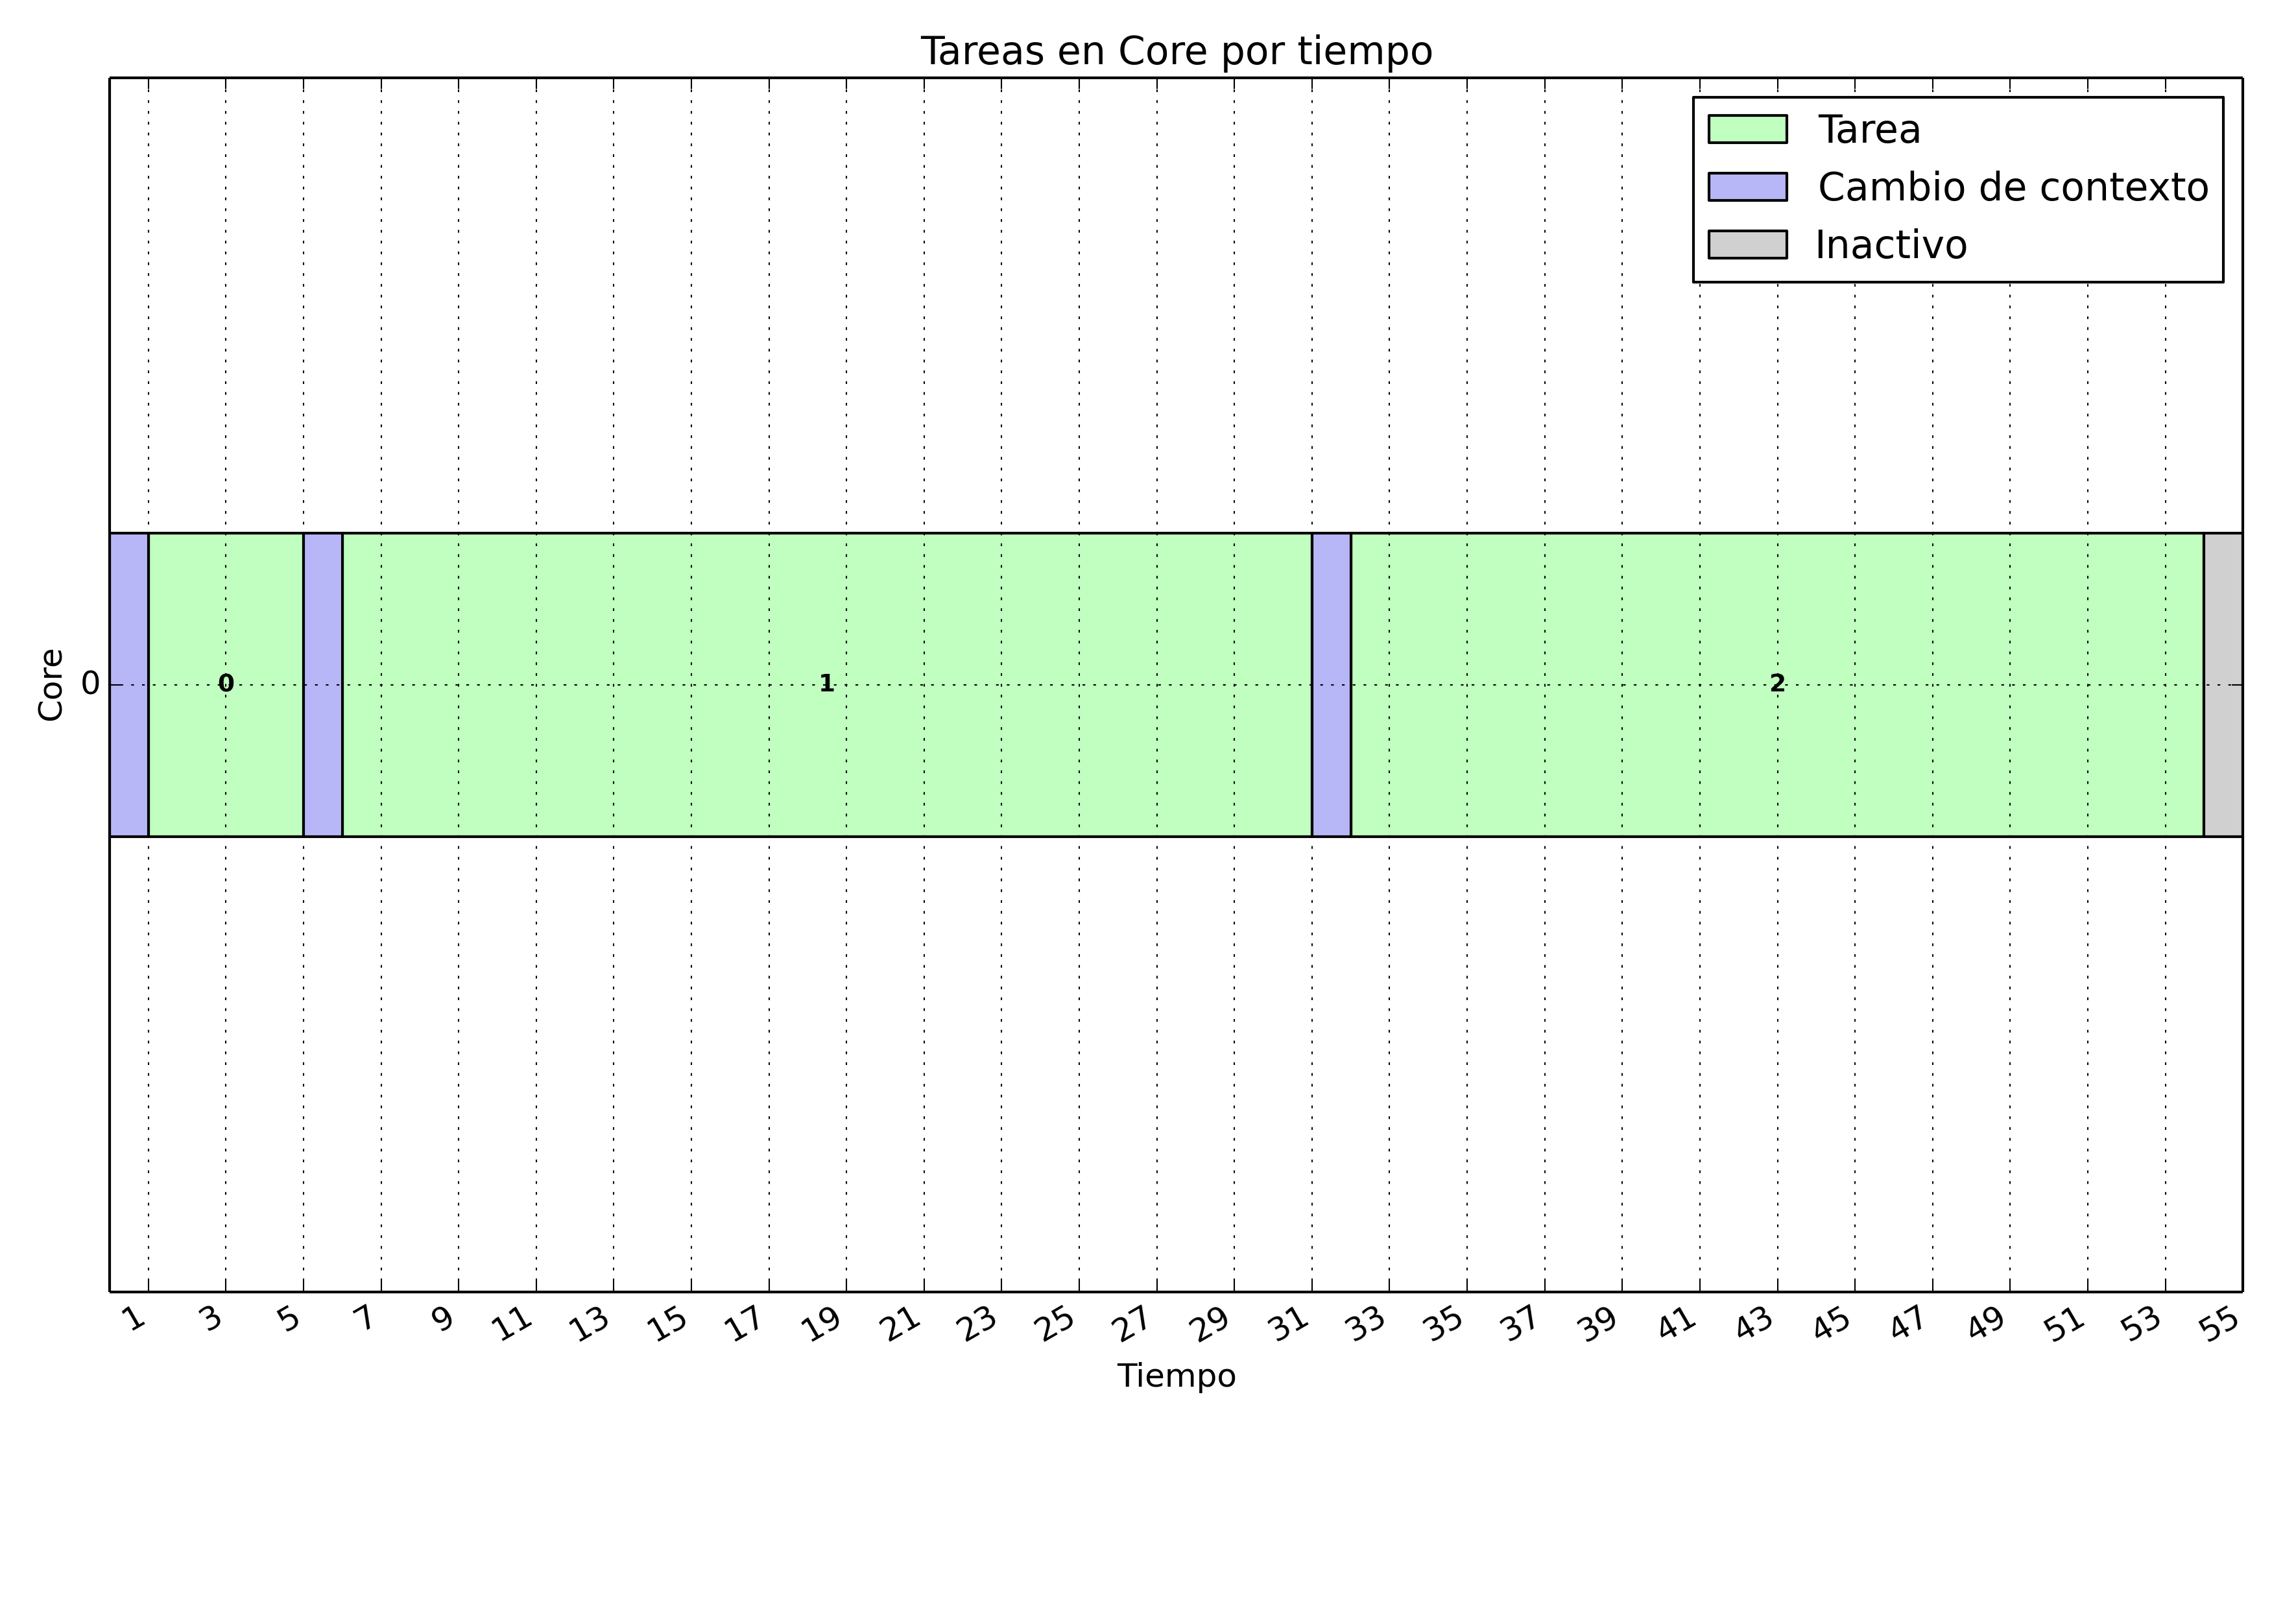
\includegraphics[width=\textwidth]{ejercicio_2_1}
\end{figure}

\begin{figure}[H]
\caption{1 TaskCPU y 2 TaskConsole con 2 cores}
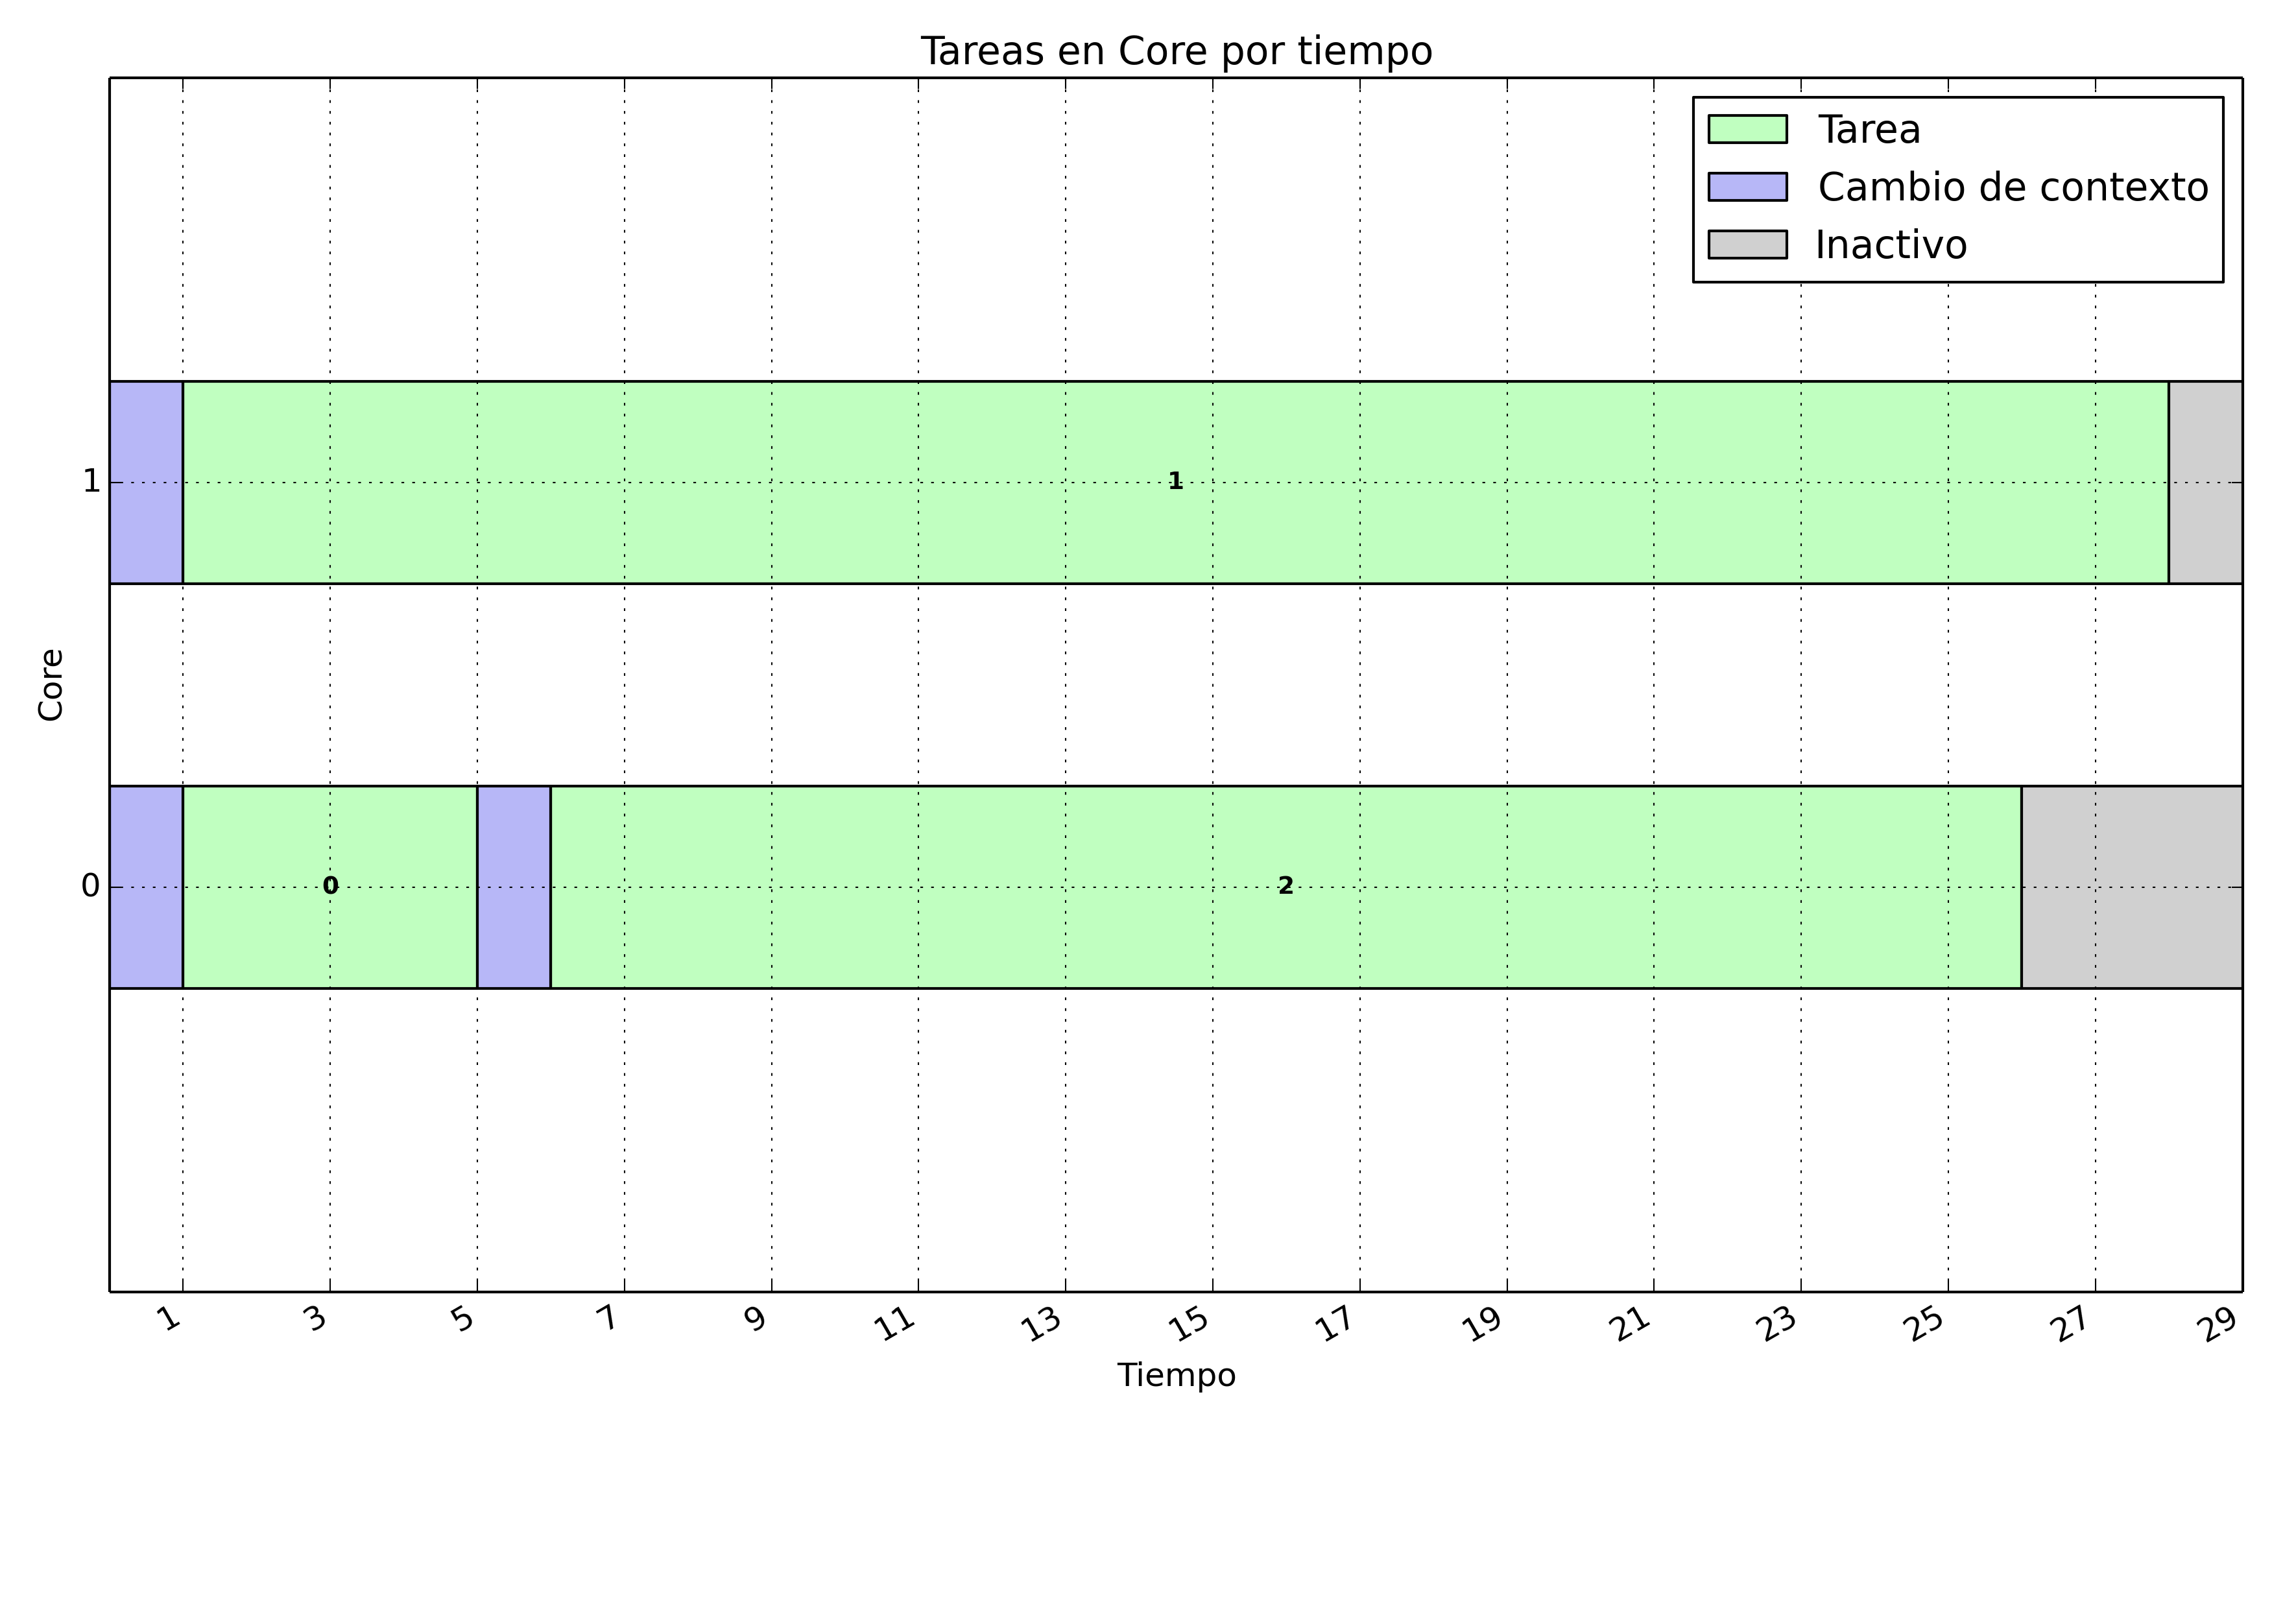
\includegraphics[width=\textwidth]{ejercicio_2_2}
\end{figure}

\begin{figure}[H]
\caption{1 TaskCPU y 2 TaskConsole con 3 cores}
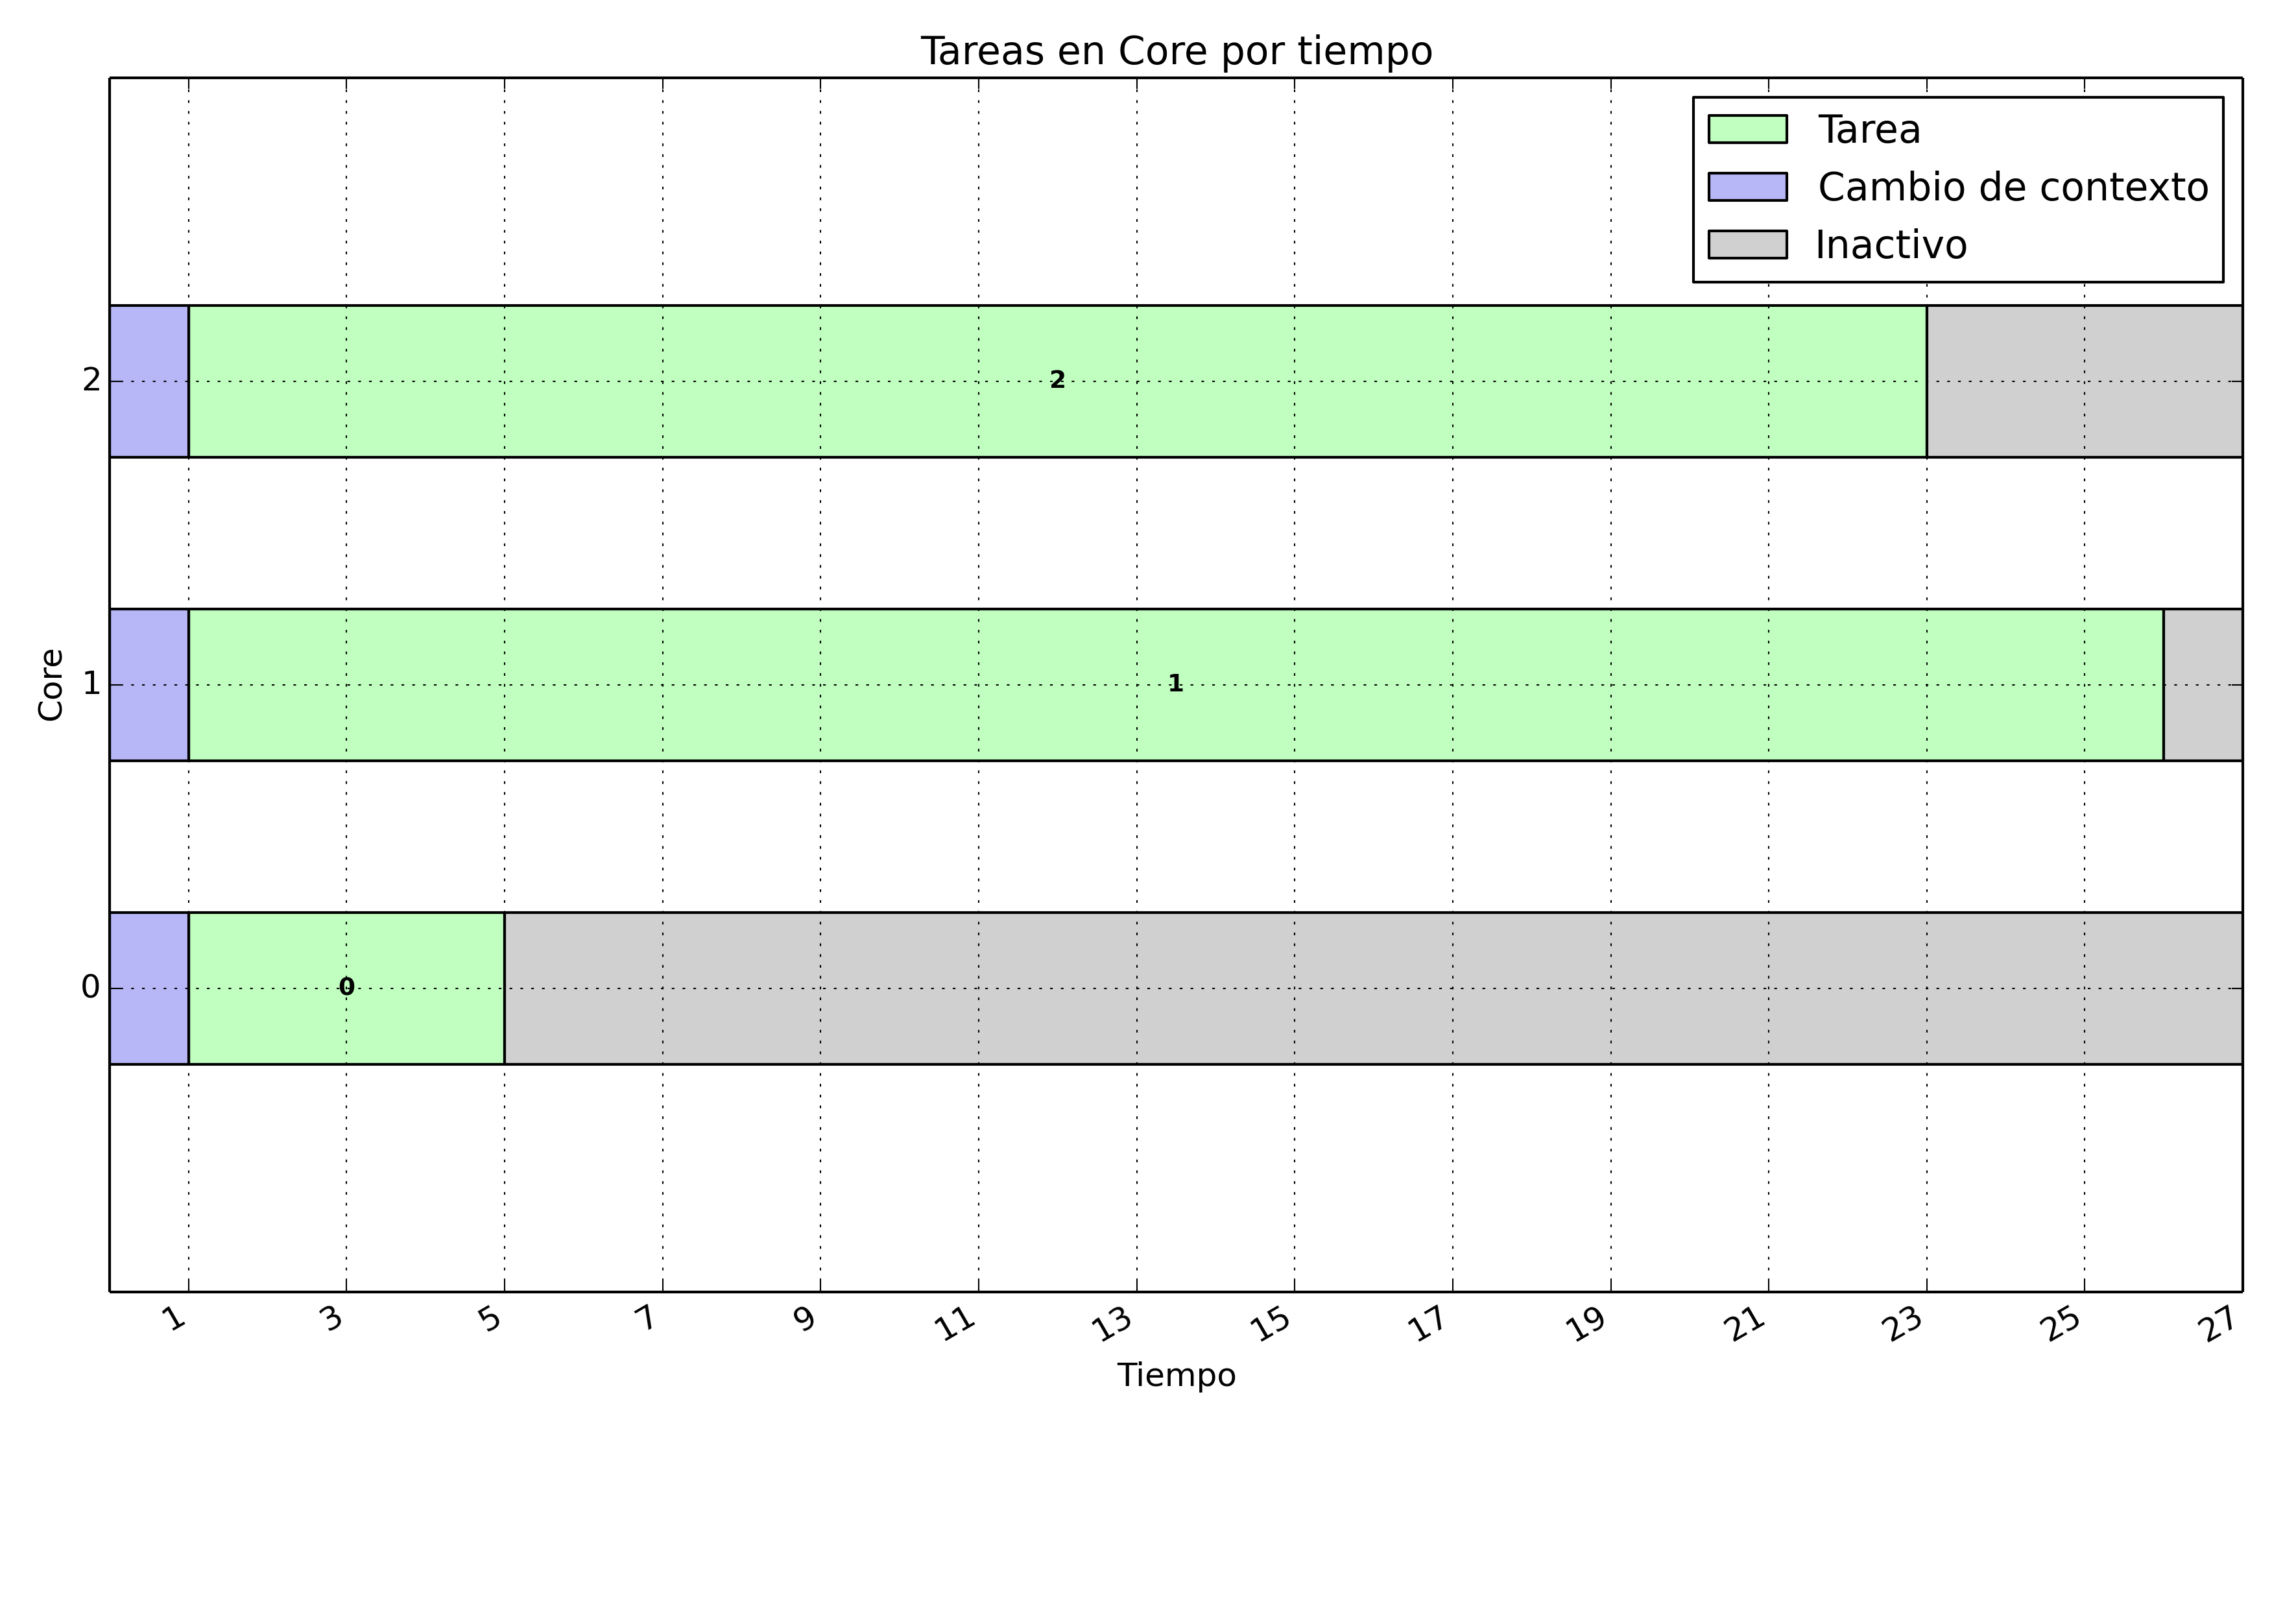
\includegraphics[width=\textwidth]{ejercicio_2_3}
\end{figure}

Se observa que no hay desalojo en esta estrategia de scheduling. De manera que cada vez que a una tarea se le concede el recurso CPU no lo libera hasta que termina su ejecuci\'on independientemente de los bloqueos que realice. Esto se implement\'o en el c\'odigo no realizando ninguna l\'ogica en la funci\'on que maneja el evento block. 

\begin{verbatim}
void SchedFCFS::unblock(int pid) {
    // Uy! unblock!... bueno, ya seguir'a en el próximo tick
}
\end{verbatim}

Observemos qu\'e sucede si las primera tareas que toman el procesador es la que que tarda m\'as en terminar. Usemos el siguiente lote, ejecutado en un core :

\begin{verbatim}
TaskConsola 3 5 10
TaskConsola 3 5 10
TaskCPU 1
\end{verbatim}

\begin{figure}[H]
\caption{1 TaskCPU de poca duraci\'on y 2 TaskConsole con 1 core}
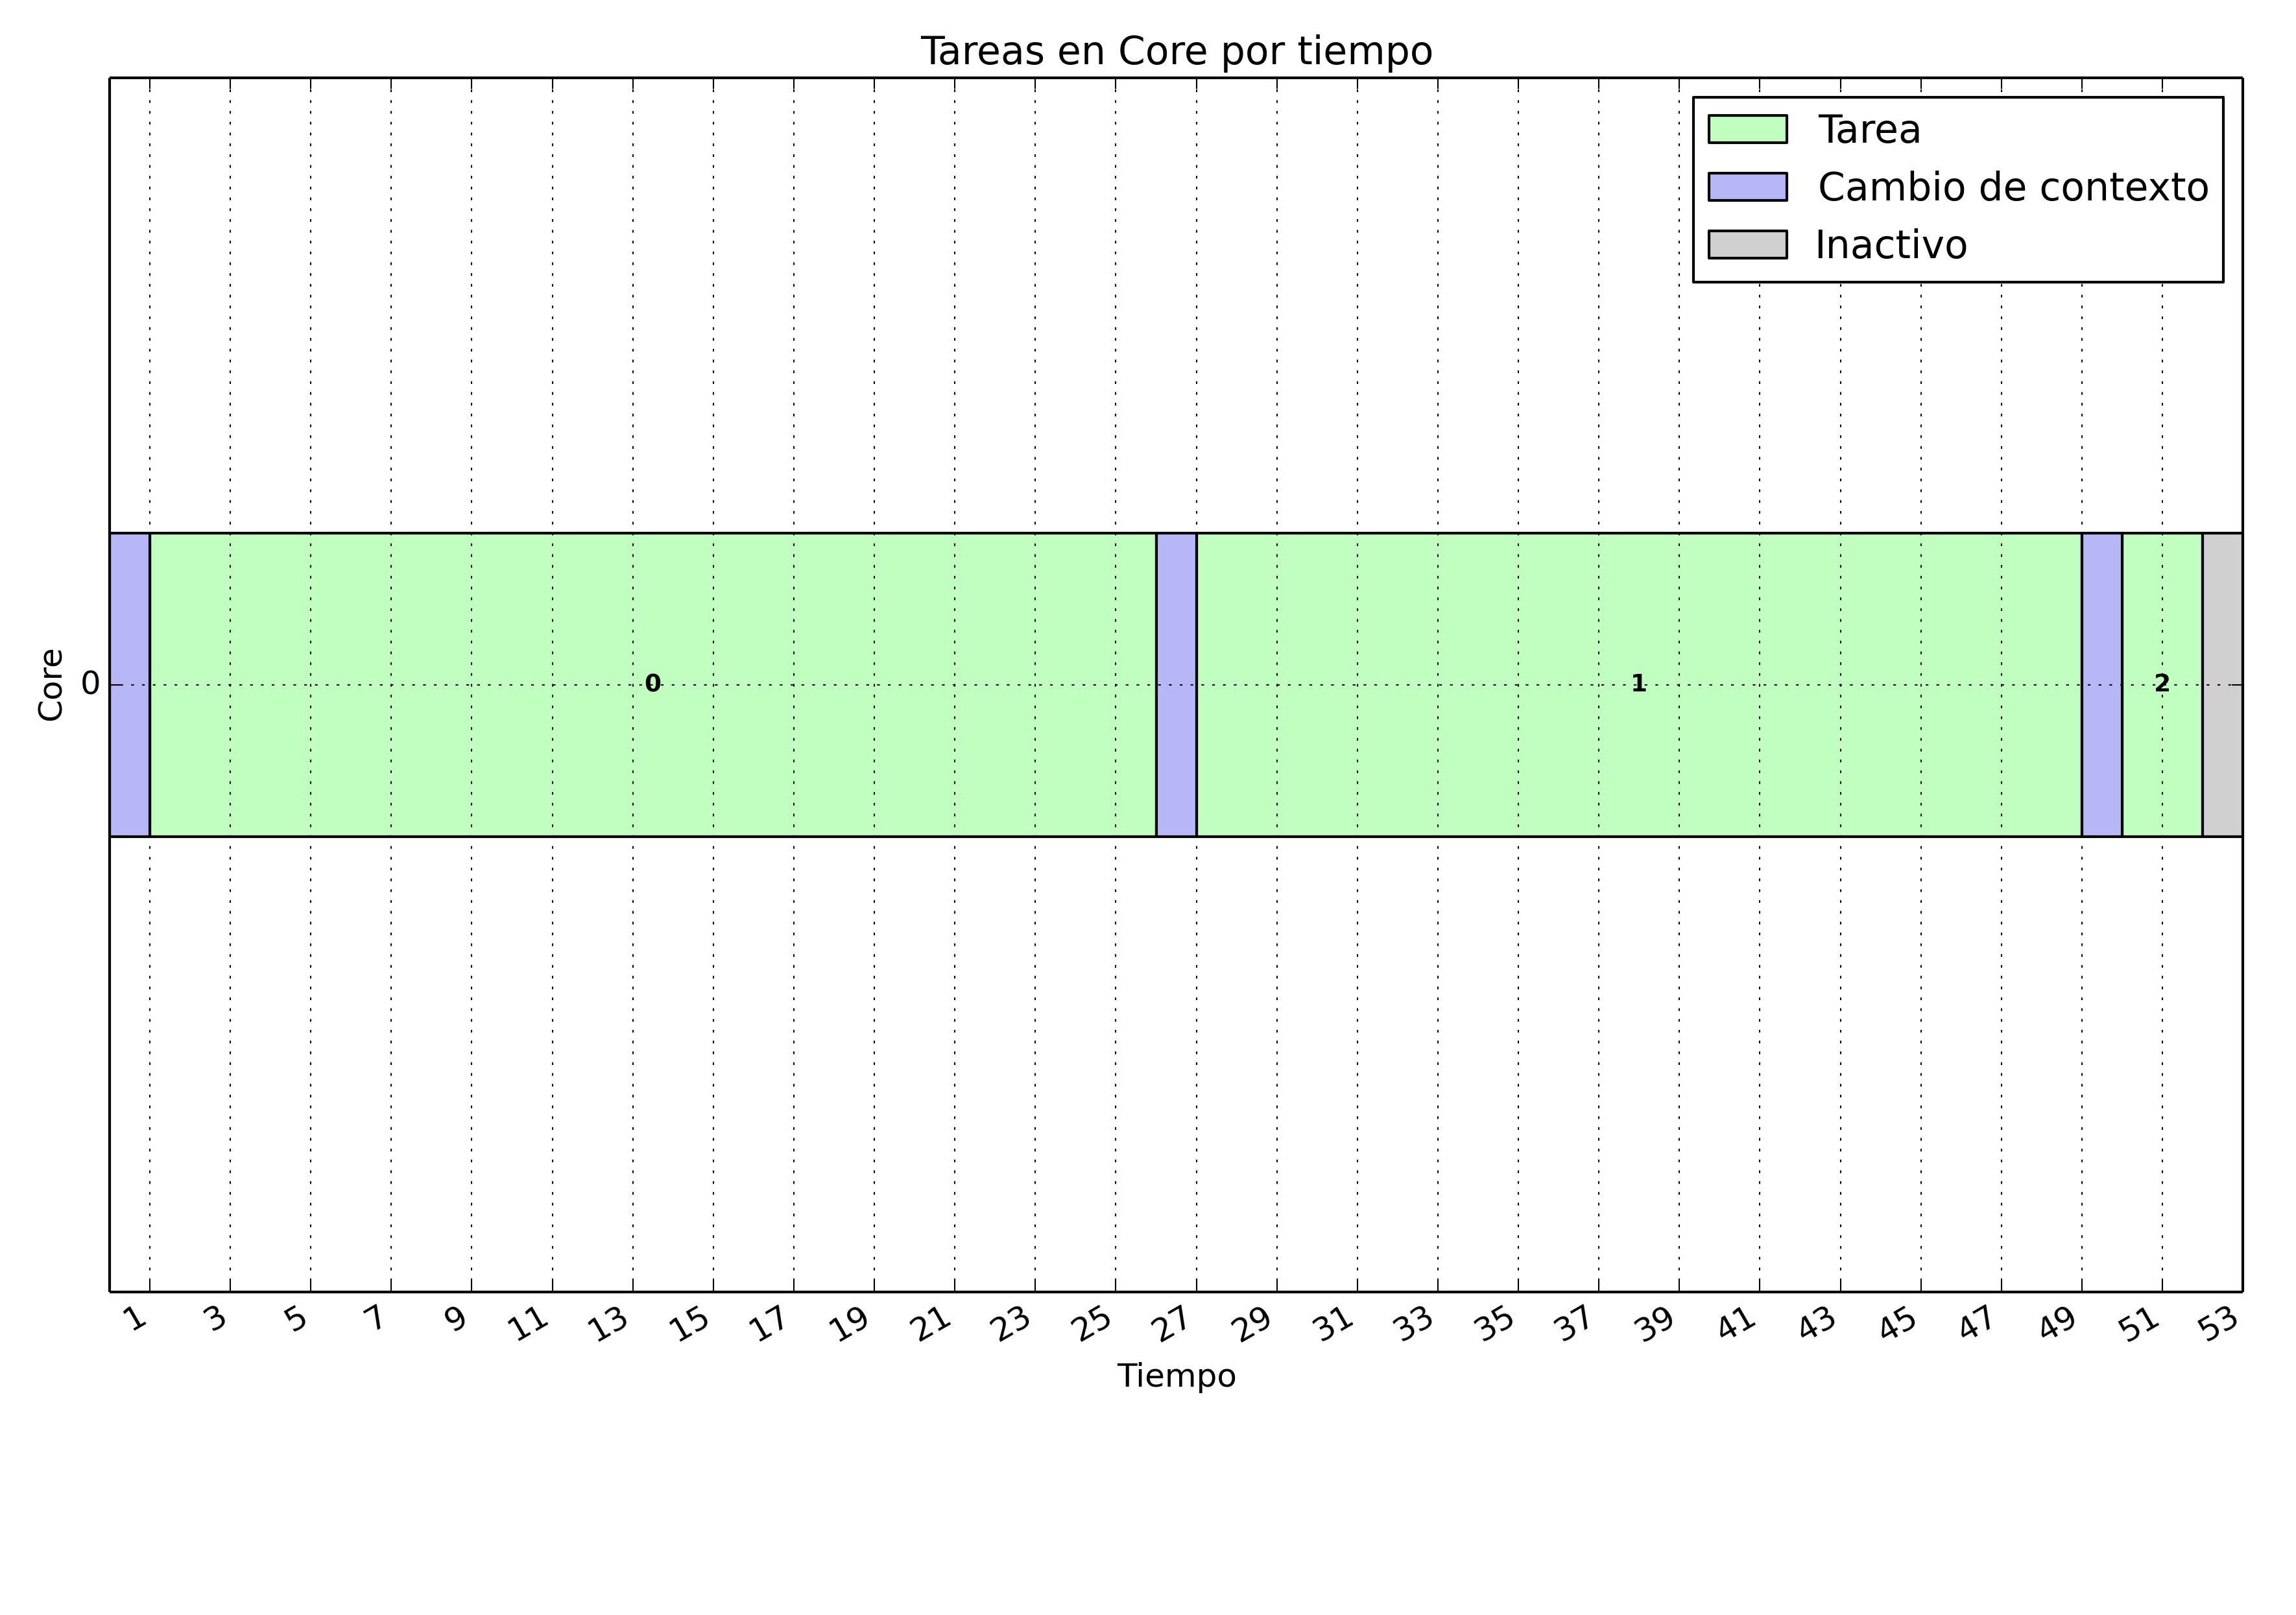
\includegraphics[width=\textwidth]{ejercicio_2_4}
\end{figure}

Como señalan varios autores \cite[p.~414]{stallings2008} \cite[p.~134]{tanenbaum2001}, este tipo de estrategias de scheduling funciona mejor para procesos cortos que para procesos de larga duraci\'on. Observamos en el lote anterior, que la tarea 3 tuvo un \textit{waiting time} de 49 ticks de reloj. Esto se aten\'ua en los lotes en los que se puede enviar la tarea a otro procesador. FCSF no parece muy atractivo para el modelo de \'unico core.

\newpage
\section{Round Robin}

Con esta nueva estrategia, podemos enfrentar el problema que tiene FCFS con las tareas de corta duraci\'on. SchedRR es el primer algoritmo que presentamos en el trabajo que usa desalojo. Cada vez que se produce un click de reloj, el algoritmo decide cu\'al es la tarea a la que se le asigna el procesador.

En la primera de las estrategias \textit{round robin}, de acuerdo a lo solicitado en el \textbf{ejercicio 3}, se usa una \'unica cola global. Cuando una tarea est\'a lista para ejecutarse pasa a esta cola, a la que llamaremos cola de ready. 

Peri\'odicamente, cuando se produce la interrupci\'on de reloj, se verifica si finaliz\'o el quantum del n\'ucleo correspondiente. Si es as\'i, la estrategia toma el primer elemento de la cola, lo saca de ella y le asigna el procesador. En caso de que la cola se encuentre vac\'ia, se ejecuta la tarea IDLE. La tarea que se encontraba ejecutando, si todav\'ia no termin\'o, se vuelve a encolar.

Cuando una tarea se bloquea por pedido de E/S, sale de la cola de READY. Reci\'en vuelve a encolarse cuando se desbloquea.

Esta estrategia se encuentra implementada en los archivos \verb+sched_rr.h+ y \verb+sched_rr.cpp+. La cola se define en el header como un atributo privado:

\begin{verbatim} 
std::queue<int> q;
\end{verbatim}

Tenemos atributos que nos sirven para manejar los quantums correspondientes a cada n\'ucleo:

\begin{verbatim}
        std::vector<int> contadorQuantums; // se usa para controlar los quantums
       std::vector<int> contadorQuantumsOriginal; // guardo la cantidad de 
               // quantums de cada nucleo
\end{verbatim}

contadorQuantums lo utilizaremos para saber en cada tick de reloj si se termin\'o el quantum, mientras que contadorQuantumsOriginal es un vector que guarda para cada n\'ucleo la cantidad de ticks (interrupciones de reloj) que abarca el quantum. 

El comportamiento frente al tick de reloj se define en la funci\'on \textit{tick}.

En caso de que el proceso desalojado termine, se toma el pr\'oximo en la cola. Si la cola est\'a vac\'ia, se retorna la \verb+TASK_IDLE+:

Esta funci\'on se ocupa tambi\'en de volver el contador del quantum del n\'ucleo correspondiente al valor original en caso de que el proceso salga o se bloquee, mientras que si el proceso se encuentra todav\'ia ejecut\'andose se fija si se agot\'o el quantum.

\begin{verbatim}
    if (m == EXIT) {
        // Si el pid actual terminó, sigue el proximo encolado
        if (q.empty()) return IDLE_TASK; // si la cola esta vacia, se retorna IDLE_TAS
        else {
            int sig = q.front(); q.pop(); // sino se toma el primero y se desencola
            return sig;
         }
    } 
\end{verbatim}

En el caso de que el proceso desalojado se bloquee por E/S, se sigue el mismo comportamiento:

\begin{verbatim}
    if (m == BLOCK) {
         if (!q.empty()) { // en caso de bloqueo se usa la misma estrategia
            int sig = q.front(); q.pop();
            return sig;
         } else {
             return IDLE_TASK; // si el único proceso está bloquedo
                             // ejecuta IDLE_TASK
         }
    }
\end{verbatim}

Si la tarea no termin\'o, se realiza lo mismo pero se vuelve a encolar la tarea desalojada:

\begin{verbatim}
    if (m == TICK) {
        if (!q.empty()) { // si se produjo una interrupcion de reloj se hace lo mismo
                   // pero se vuelve a encolar la tarea
            int sig = q.front(); q.pop();
            int des = current_pid(cpu);
            if (des != IDLE_TASK) {
                q.push(des); // vuelvo a encolar el proceso desalojado
            }
            return sig;
         } else {
               return current_pid(cpu);
         }
   }
\end{verbatim}

De acuerdo a lo pedido en el \textbf{ejercicio 4}, presentamos varios lotes de tareas, observ\'ando como el comportamiento se corresponde a la estrategia \textit{round robin}:


\begin{verbatim}
TaskCPU 3
TaskCPU 3
TaskCPU 3
TaskCPU 3
TaskCPU 3
\end{verbatim}

\begin{figure}[H]
\caption{5 TaskCPU sin llamadas de E/S, 1 core}
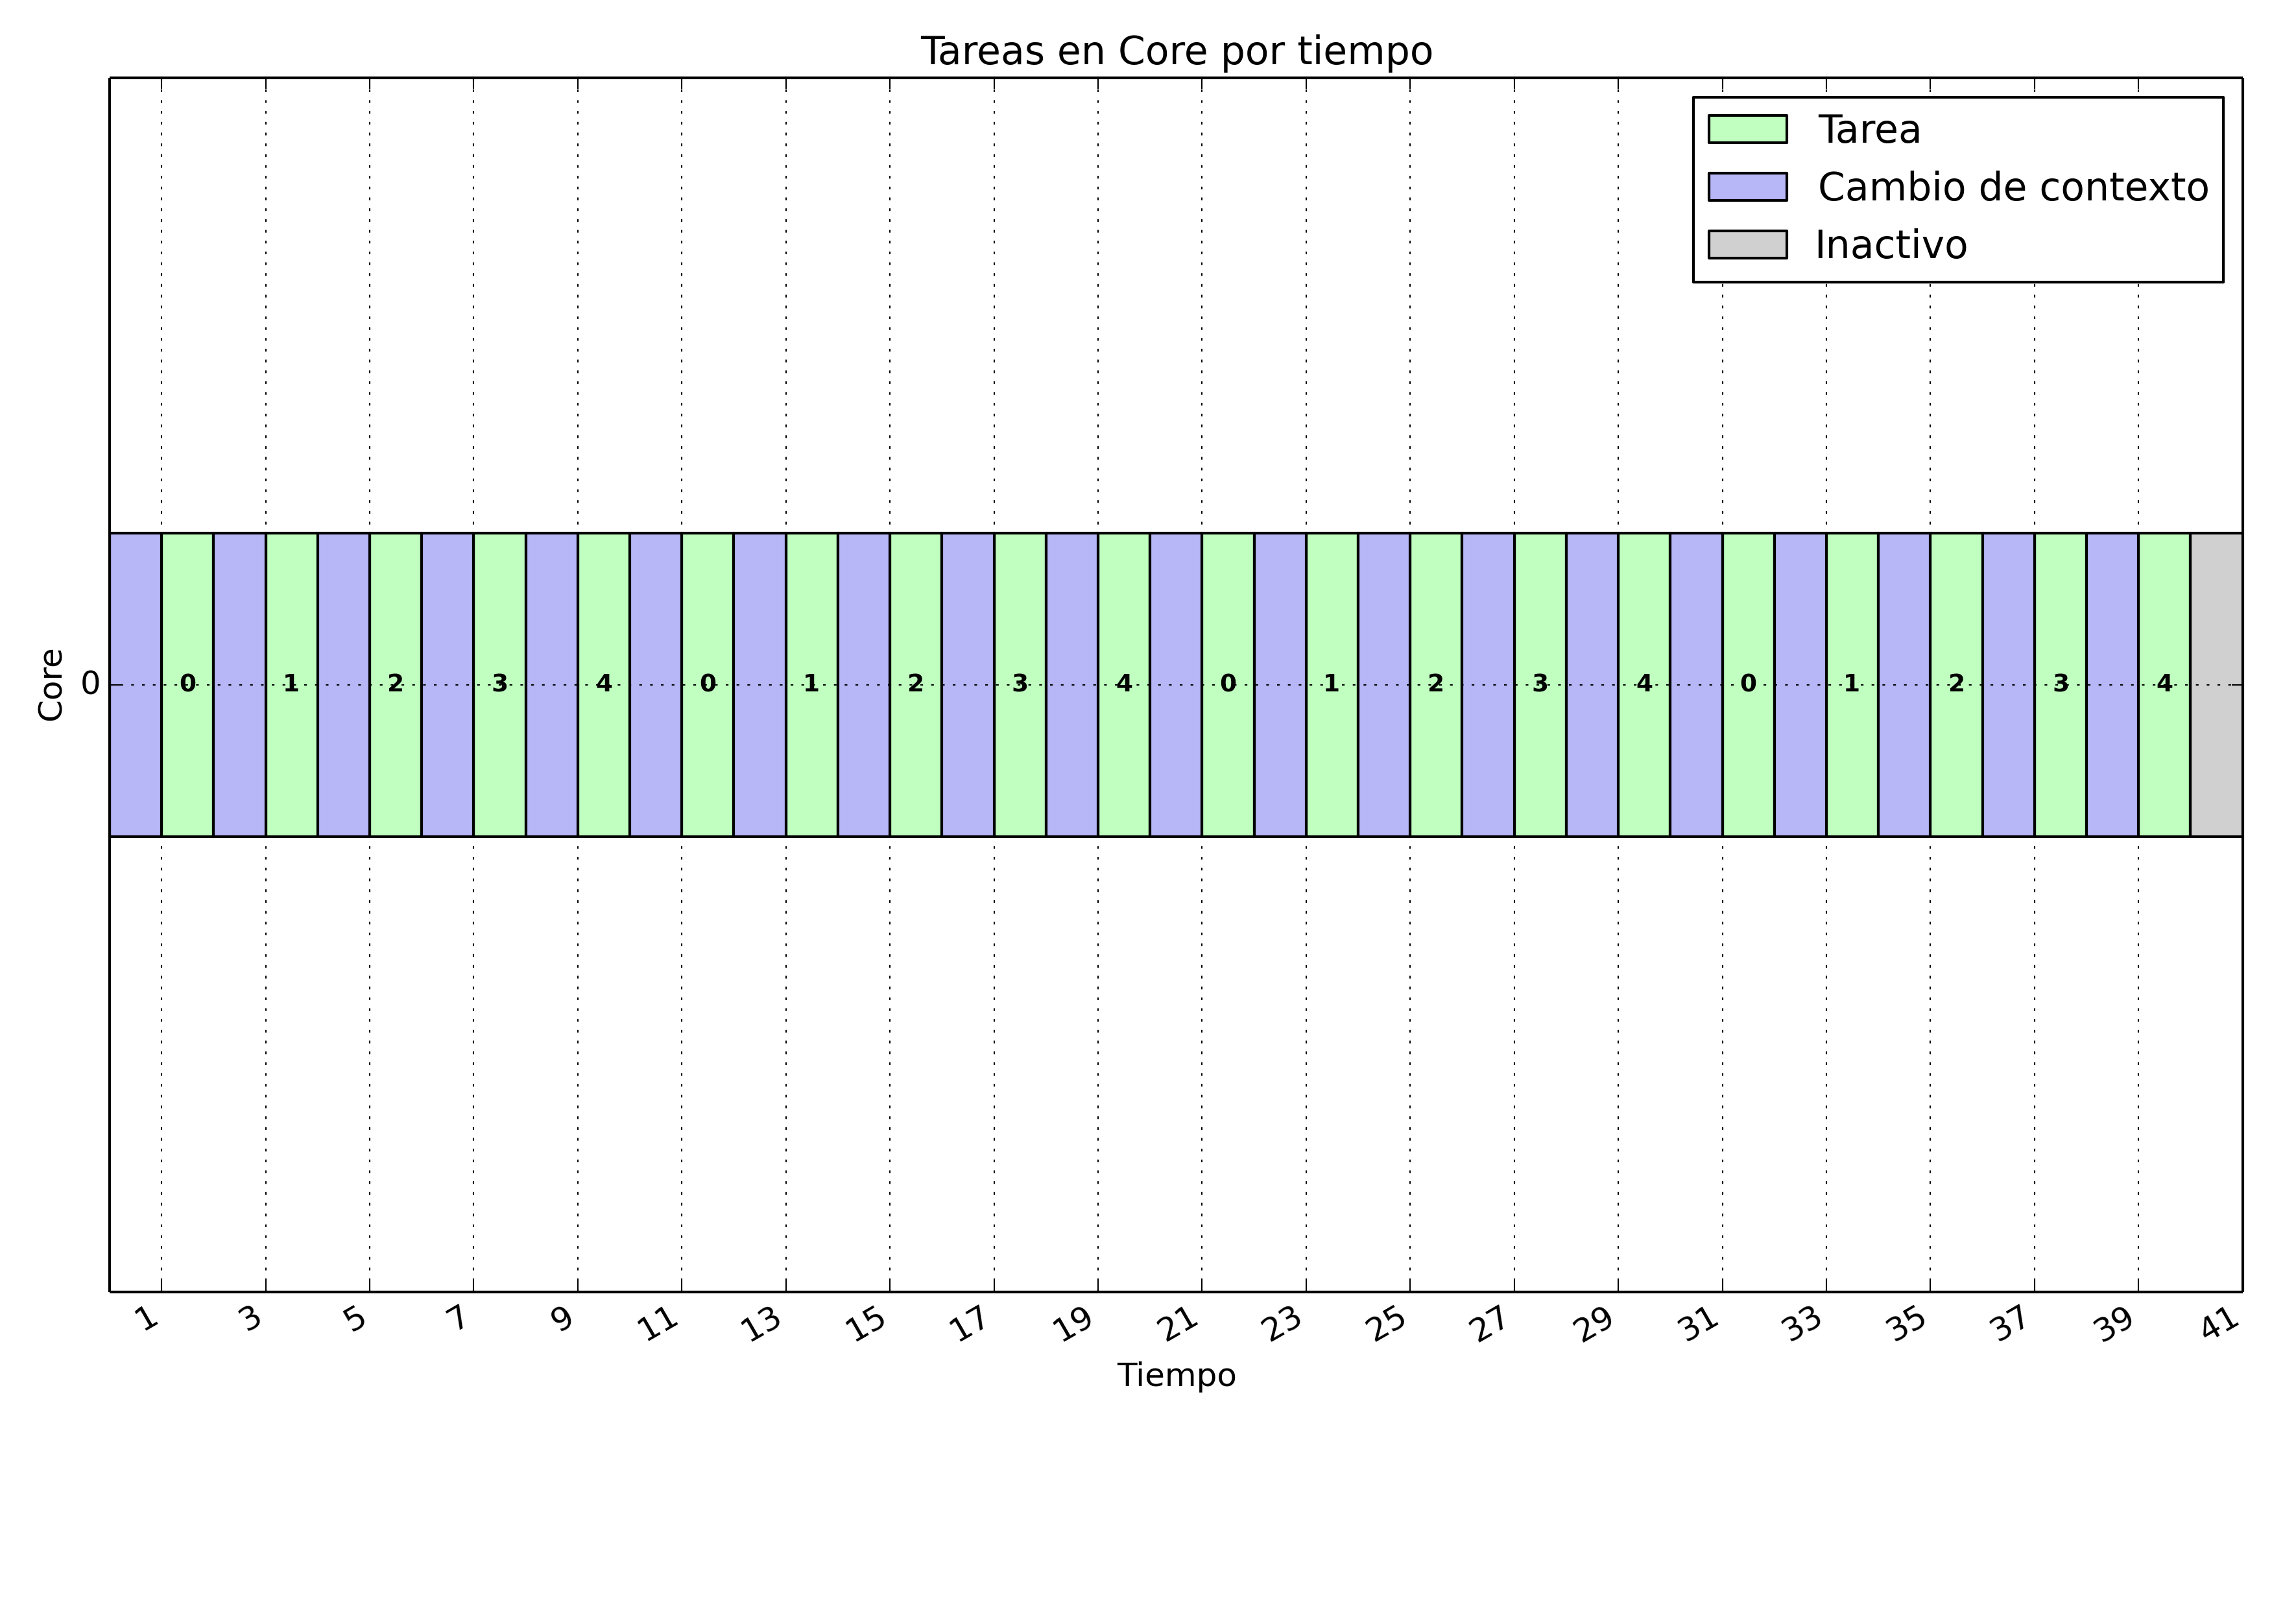
\includegraphics[width=\textwidth]{ejercicio_4_1}
\end{figure}

En este lote, se observa c\'omo act\'ua round-robin en un ambiente de un solo core. Las tareas se van alternando en el uso del procesador, con el tiempo necesario para el cambio de contexto. Cada vez que una tarea es desalojada, se vuelve a encolar hasta terminar su procesamiento. En este caso en particular, no se produjo ninguna llamada a E\S: cuando la tarea es desalojada vuelve en el mismo acto a la cola de READY. Vemos, entonces que la secuencia de ejecuci\'on fue: \verb+1-2-3-4-1-2-3-4...+

Ejecutamos el mismo lote pero con dos cores:

\begin{figure}[H]
\caption{5 TaskCPU sin llamadas de E/S, 2 cores}
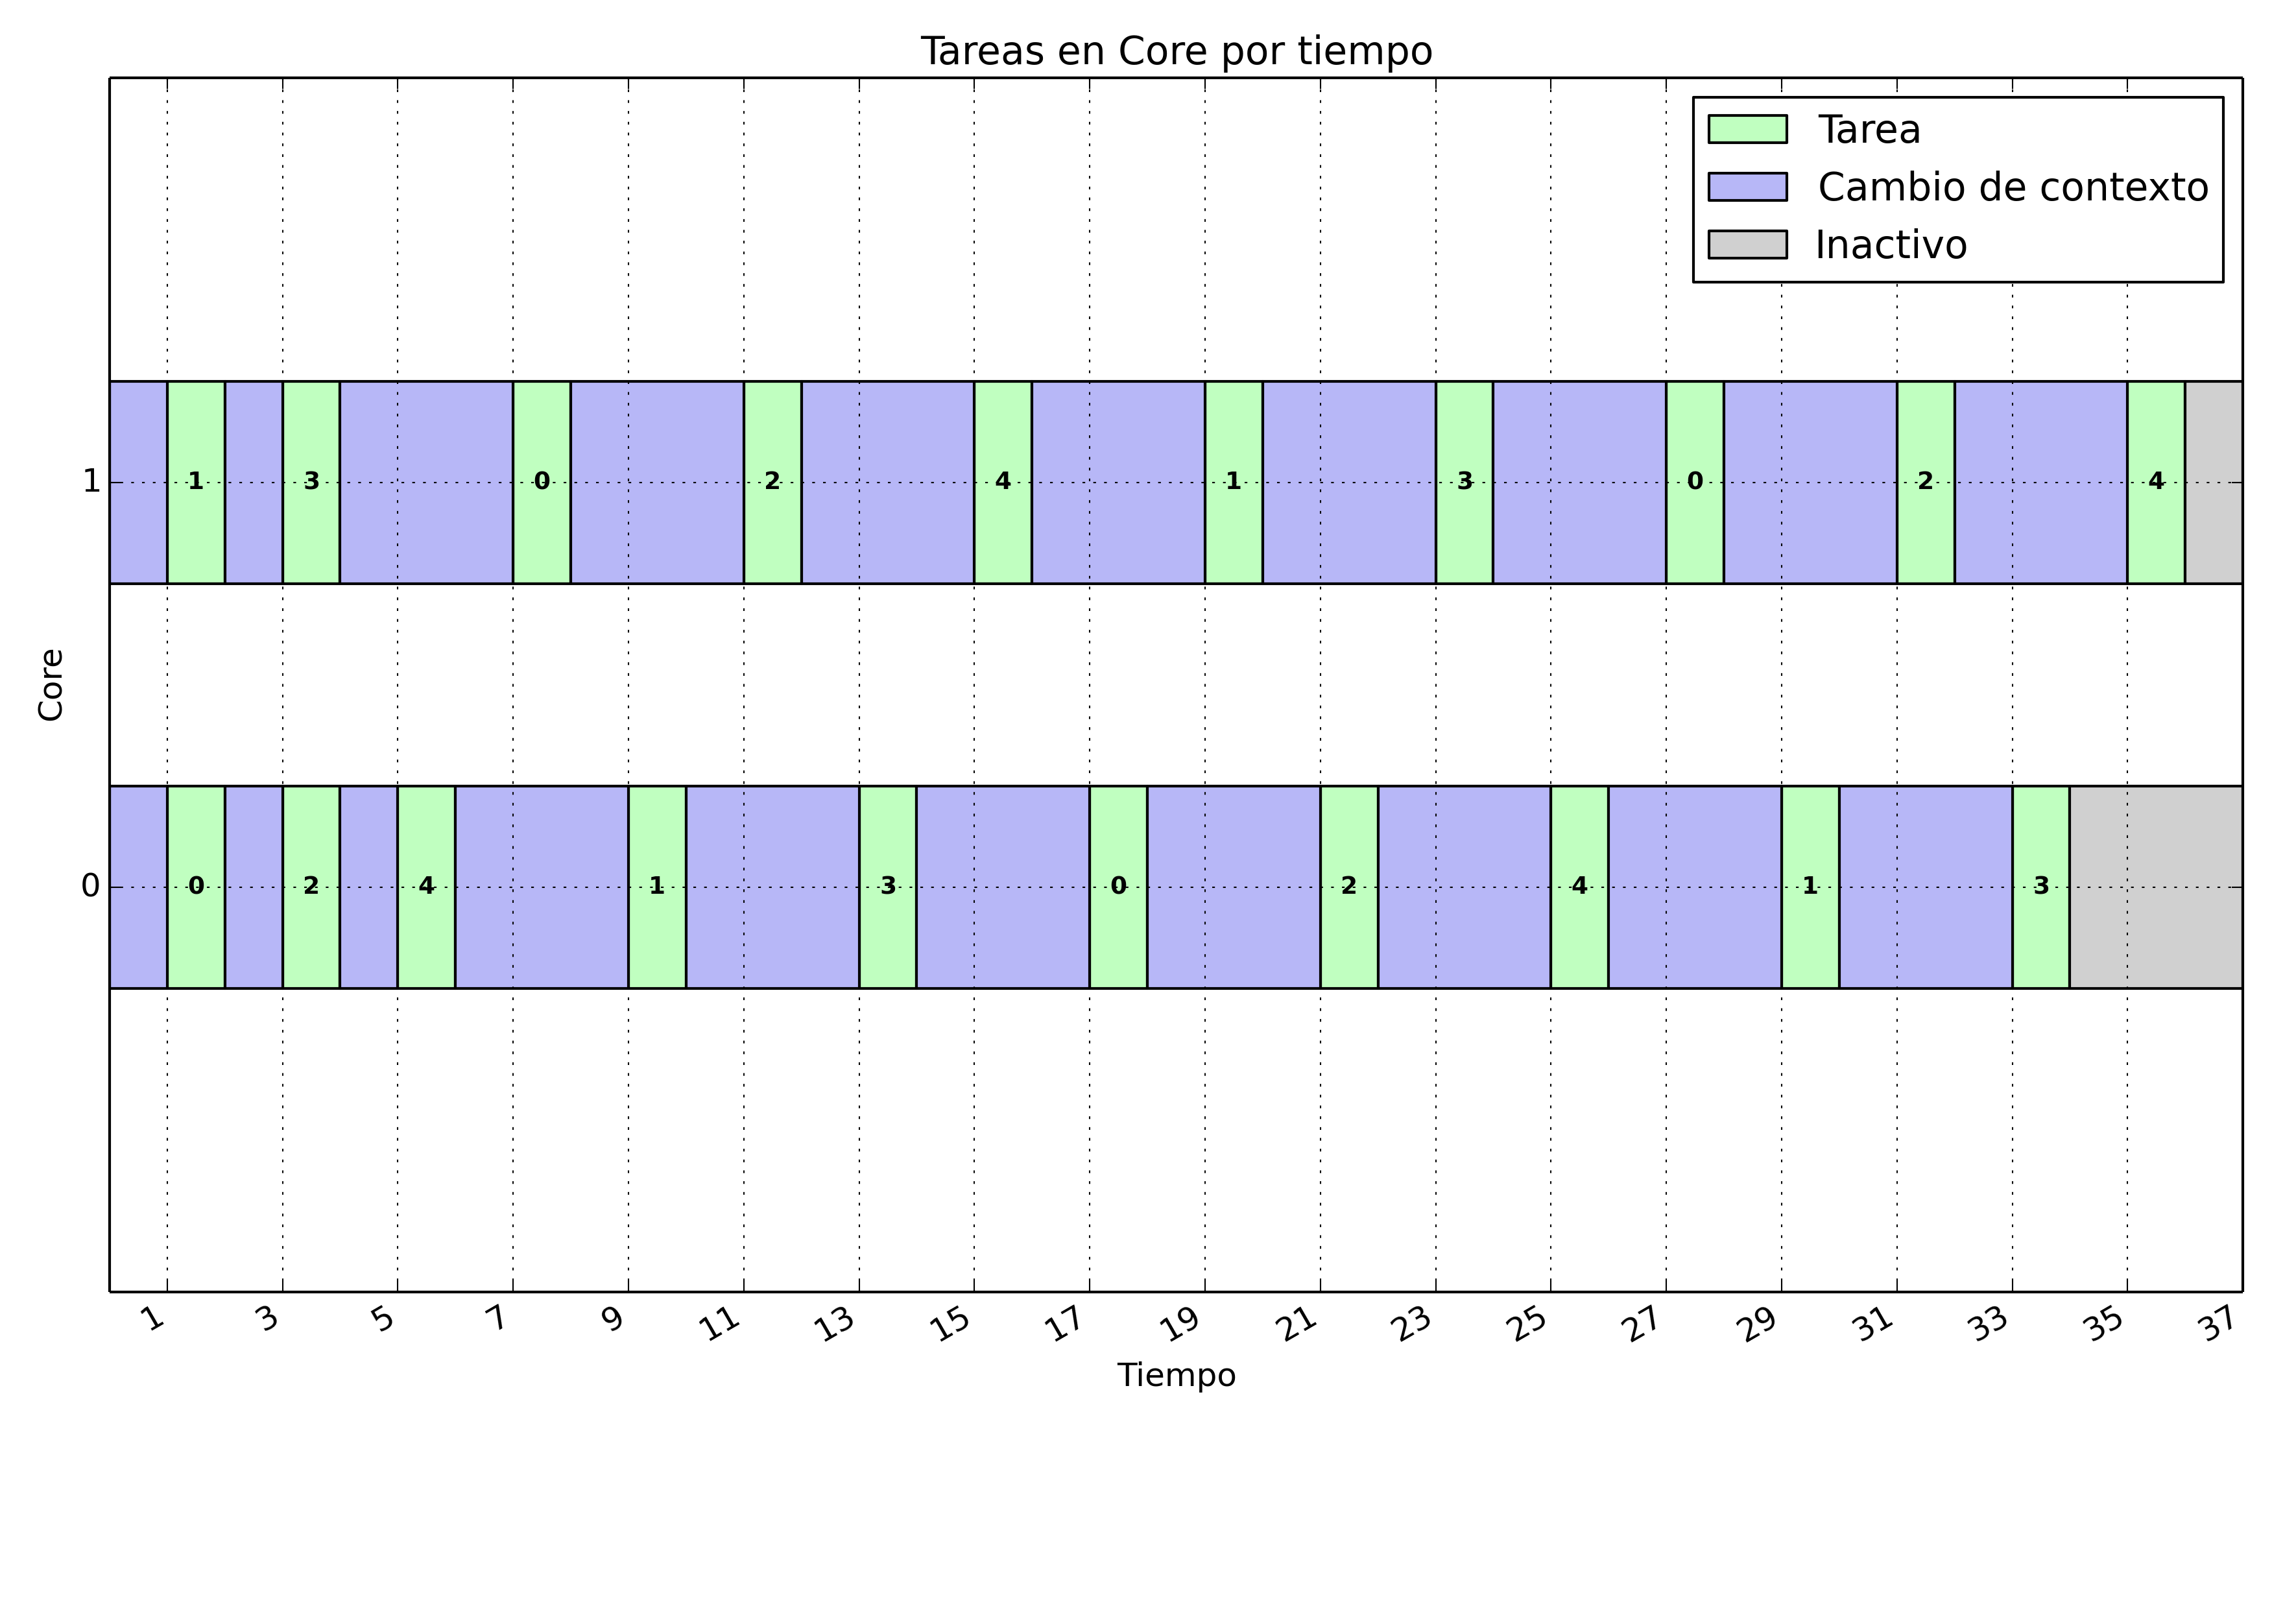
\includegraphics[width=\textwidth]{ejercicio_4_2}
\end{figure}

En este caso, vemos como al tener una \'unica cola global, se produce el pasaje de una tarea de un core a otro. 

Se debe notar que hasta al tick 4 de reloj, entre el quantum de cada tarea, nada m\'as tenemos el overhead del cambio de contexto. Sin embargo, al pasar las tareas a los otros cores, el overhead entre tarea aumenta ya que le pedimos que el cambio de core tome 2 ticks de reloj. Esta primera versi\'on de \textit{round robin} no toma en cuenta la penalidad de cambio de n\'ucleo, por lo que cuando se toma una tarea de la cola no se toma en cuenta si estuvo ejecutando en el otro core.

De todos modos, vemos como se contin\'ua globalmente la idea de una cola circular. La selecci\'on de la tarea asignada al core del tick sigue teniendo la secuencia \verb+1-2-3-4-1-2-3-4...+

Por \'ultimo, tomamos un lote con una tarea que llama a E/S y se bloquea:

\begin{verbatim}
TaskCPU 3
TaskConsola 3 5 10
TaskCPU 3
TaskCPU 3
TaskCPU 3
TaskCPU 3
\end{verbatim}

\begin{figure}[H]
\caption{5 TaskCPU y un TASKCONSOLE que llama a E/S, 1 core}
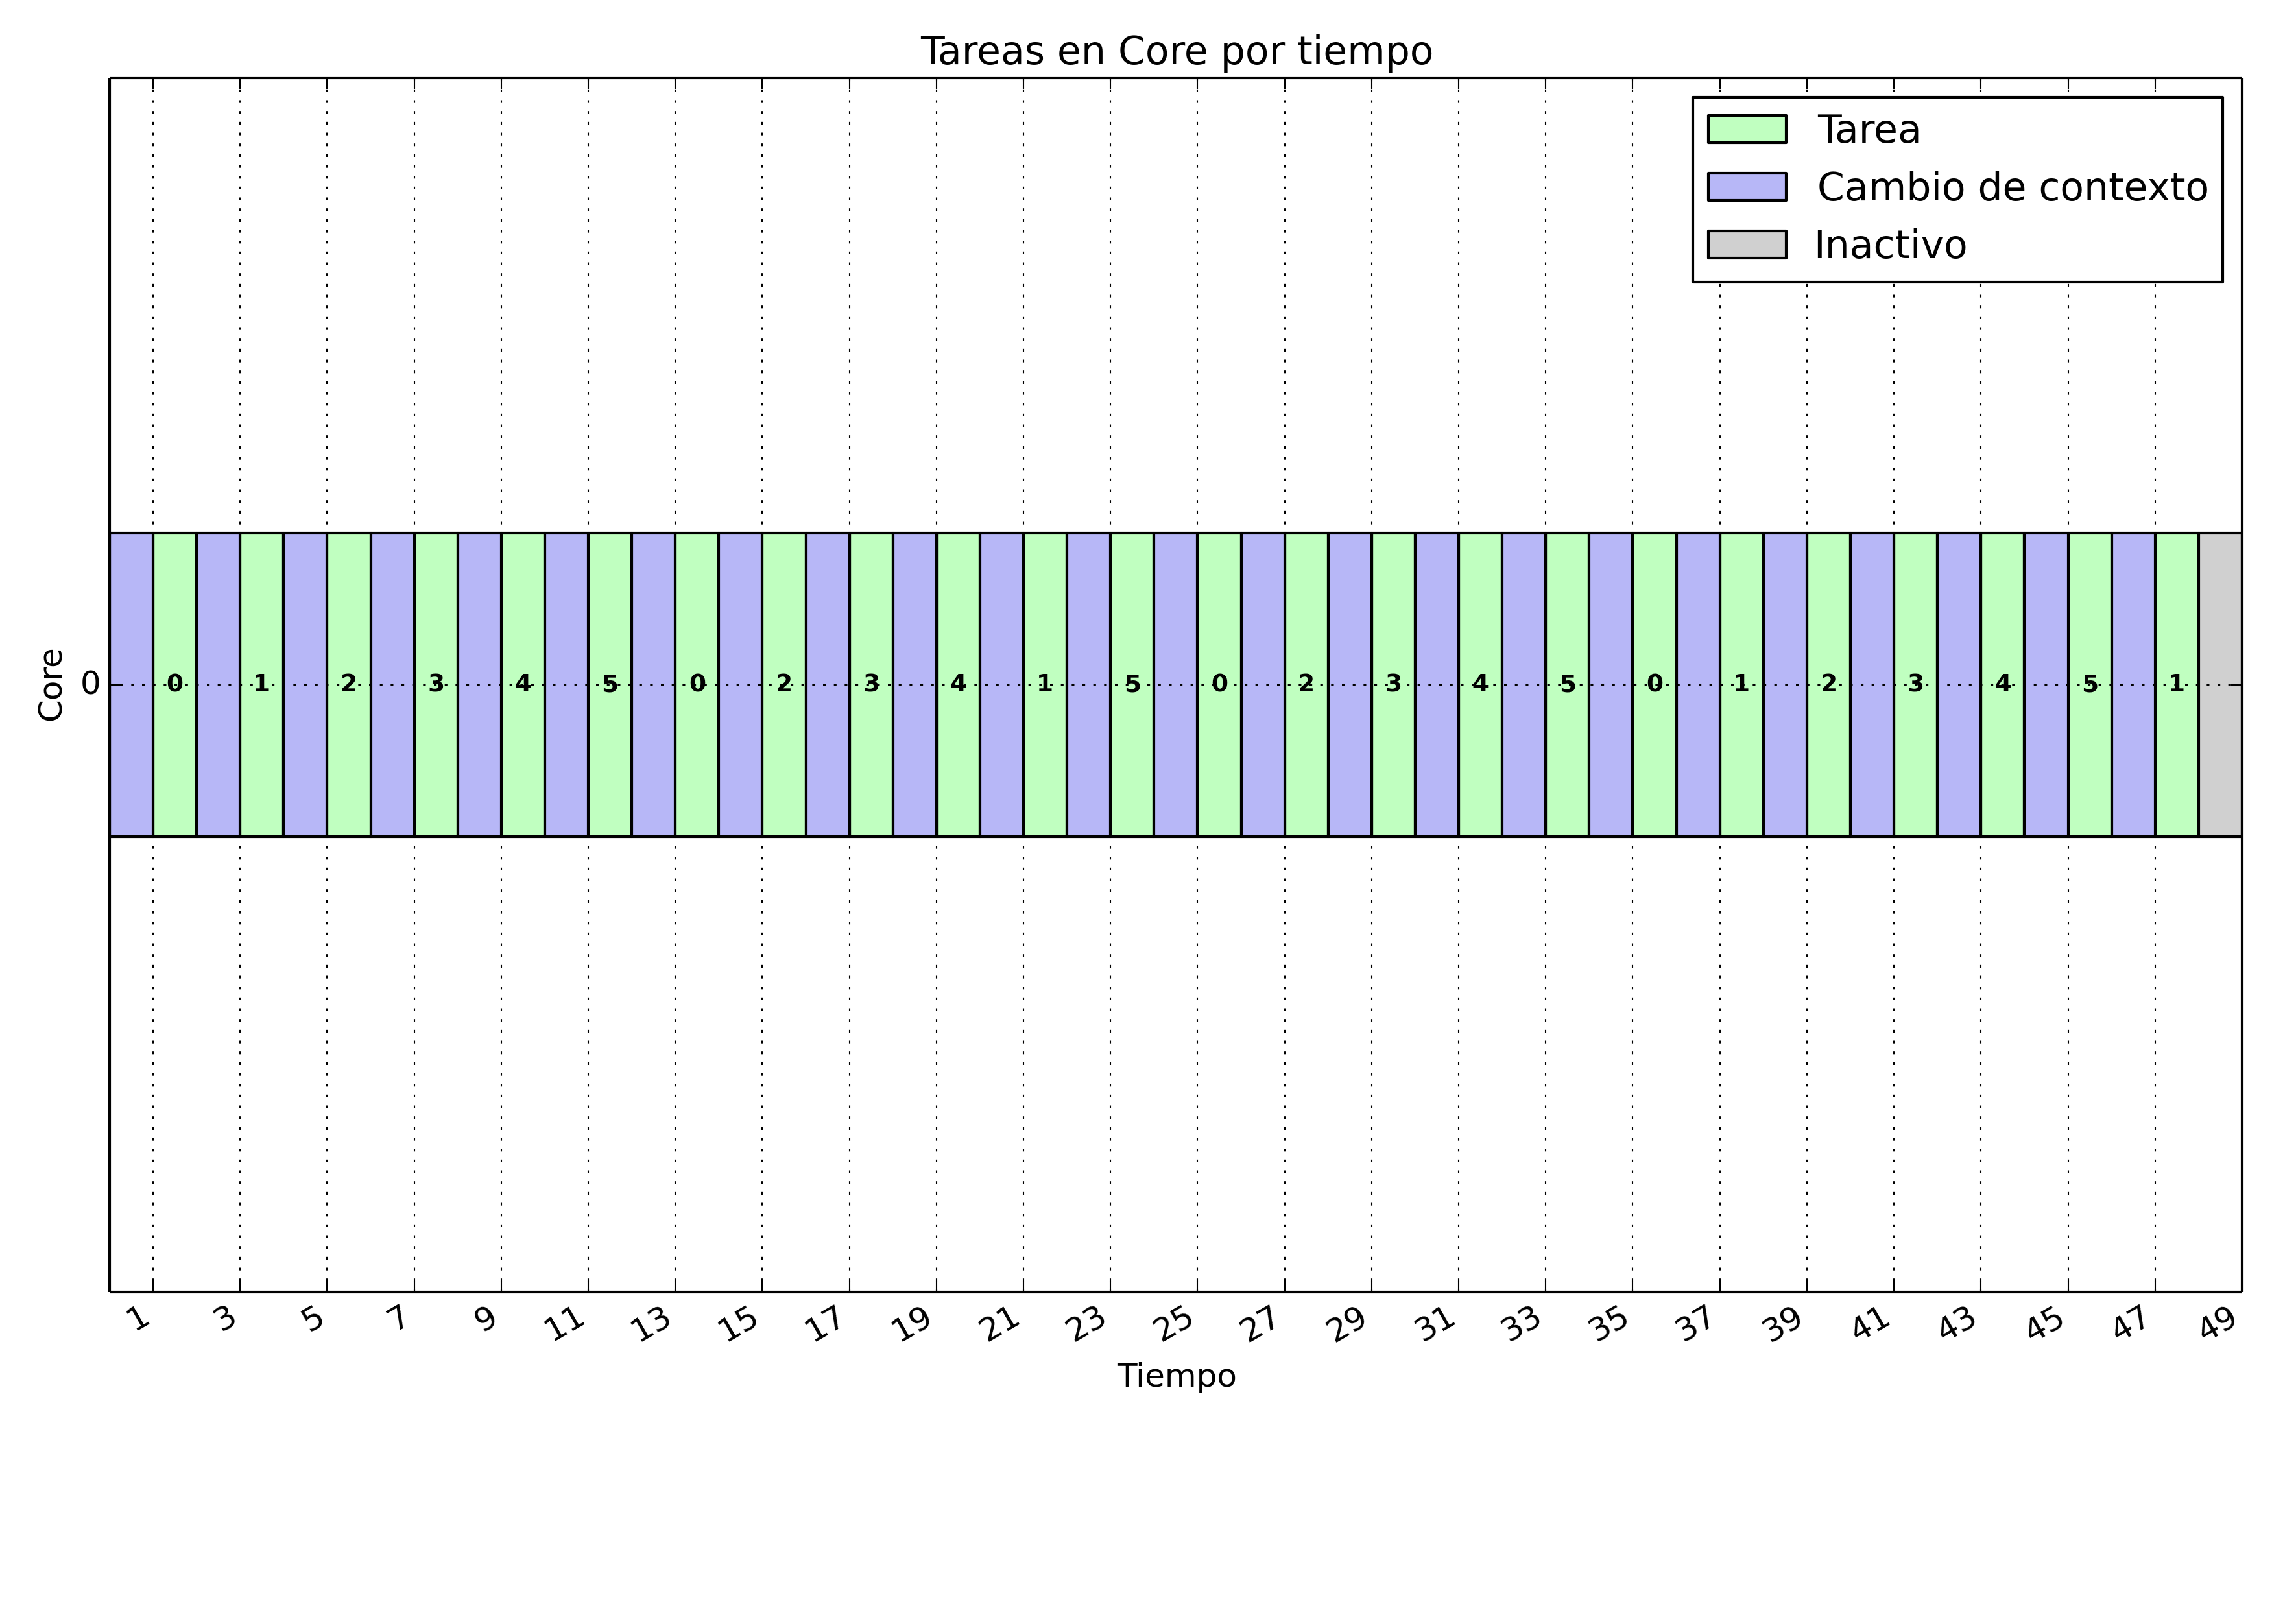
\includegraphics[width=\textwidth]{ejercicio_4_3}
\end{figure}

Observemos que en este caso la tarea 1 se bloquea y no veulve a la cola hasta tick 22.

\newpage
\section{Scheduling para tiempo real}

Al analizar los algoritmos de scheduling, Tanembaum \cite[p.~136]{tanenbaum2001} señala que es relevante distinguir tres ambientes diferentes:

\begin{itemize}
	\item{Batch}
    
    \item{Interactivo}
    
    \item{Tiempo Real}
\end{itemize}

En los ambientes batch, no existe la exigencia planteada por los usuarios frente a alg\'un tipo de perif\'erico o terminal. Como no se necesita una respuesta interactiva r\'apida, son aceptables algoritmos sin desalojo o bien algoritmos con desalojo que tienen un quantum largo. Se requiere un uso intensivo y largo del CPU. Conviene entonces minimizar el overhead del cambio de contexto.

En el caso de los ambientes interactivos, lo que se intenta es que las tareas no acaparen el recurso CPU e impidan que otras tareas accedan a \'el. Por ello, conviene plantear una estrategia de desalojo.

El tercer ambiente es el que concierne al paper de Liu y Leilan \cite{liuleiland1973}: tiempo real. Se trata de ambientes en los que el control del tiempo de ejecuci\'on de cada proceso es cr\'itico. En estos ambientes \textbf{es necesario que la ejecuci\'on de cada tarea termine antes de que pase un per\'iodo determinado de tiempo (deadline)\footnote{Esta es la respuesta al ejercicio 5 a}}. En caso de que no se cumpla esta restricci\'on, se producir\'a un \textit{overflow}. Esto es lo que distingue a un ambiente \textit{hard real time} de un \textit{soft real time}, en donde basta con cumplir estad\'isticamente el control de tiempo de ejecuci\'on.


Dadas las condiciones del ambiente, se hace necesario asignar alg\'un tipo de prioridad a las tareas. El paper presenta dos algoritmos: uno de \textit{prioridad fija}, que asigna a cada tarea su prioridad cuando son cargadas en el sistema, y uno de \textit{prioridad din\'amica} que asigna prioridades din\'amicamente en el momento en que el scheduler tiene que decidir qu\'e tarea va a ejecutar (cuando se termina el quantum o bien cuando el procesador queda libre por bloqueo o por terminarse la tarea que estaba ejecut\'andose). En el primer caso, las prioridades no cambian a lo largo de tiempo: se trata de un sistema de asignaci\'on de prioridades est\'atica, mientras que en el segundo caso se trata de un sistema din\'amico en cuanto a la asignaci\'on de prioridades. 

En el paper de Liu y Layland se explicitan una serie de conceptos relevantes para el problema:

\begin{itemize}
	\item \textit{T}, el \textit{request period} es el tiempo que pasa entre una ejecuci\'on de la tarea y la pr\'oxima llamada a la tarea. Se supone que el per\'iodo comprendido entre el momento en que la tarea entra al sistema y el momento en que sale, tiene que ser menor al \textit{request period} para evitar overflow.
    
    \item \textit{C}, el tiempo de ejecuci\'on o \textit{runtime}, el tiempo total en que la tarea realizar\'a operaciones en el sistema.
    
    \item el \textit{request rate}, la inversa del \textit{request period}.
\end{itemize}

El algoritmo de asignaci\'on fija  determina cu\'al es la prioridad de la tarea en el momento de la carga, asign\'andole importancia a cada proceso de acuerdo a la inversa de su request period, es decir a su \textit{request rate}.

Este algoritmo se encuentra implementado en los archivos \verb+sched_fixed.h+ y \verb+sched_fixed.cpp+.

En \verb+sched_fixed.h+ definimos la clase  TaskComparable:

\begin{verbatim}
class TaskComparable
{
  public:
     TaskComparable() {};                                      //constructor default
    TaskComparable(int pid, int priority)
    { this->pid = pid; this->period = period;}    
     bool operator<(const TaskComparable& right) const{
   
         return (this->period)  < (right.period);
    }

     int get_pid() const { return pid; }             //accessor methods
    int get_period() const { return period; }

  private:
    int pid, period;                                 //data fields
};
\end{verbatim}

Cuando una tarea entra en el sistema guardamos la informaci\'on de su per\'iodo y de su id de proceso en una instancia de esta clase, que define un operador de menor. Esto lo hacemos para poder encolarla en una \verb+periority_queue+ y as\'i mantener los procesos siempre ordenados de acuerdo al request rate (o lo que es lo mismo, darle m\'as prioridad a aquellas tareas que tenga menor request period).

El manejo del fin del quantum es similar al round-robin en la medida  en que se tomar\'a el primero de una cola de prioridad y se volver\'a a encolar el que estaba ejecutando en el caso de que no se bloquee o termine.

La \'unica diferencia es que el proceso se volver\'a a encolar en la \verb+priority_queue+ antes de obtener el siguiente proceso a aejecutar ya que el proceso que se encuentre en RUNNING puede seguir ejecutando si no entr\'o otro proceso de mayor prioridad:

\begin{verbatim}
    if (m == TICK) {
          if (!q.empty()) {
            int des = current_pid(cpu);
            if (des != IDLE_TASK) {
                TaskComparable tsk;
                tsk = TaskComparable(des, period(des));
                 q.push(tsk); // vuelvo a encolar la tarea que esta ejecutando
            }
            int sig = q.top().get_pid(); q.pop();
            return sig;
            } else {
            return current_pid(cpu);
         }
     }
\end{verbatim}

En la secci\'on 7 del paper se presenta lo que se llama el \textit{deadline driven algorithm}\footnote{Ejercicio 5 b}. Como dijimos, se trata de un algoritmo de asignaci\'on din\'amica de prioridades. Al finalizar cada quantum o al quedar libre el procesador, la estrategia de asignaci\'on del recurso no se basa en la prioridad dada en la carga de la tarea, sino que se dar\'a una mayor prioridad a aquellos procesos cuya \textit{deadline} est\'e m\'as pr\'oxima y una menor prioridad a aquellos en los que el deadline est\'e m\'as alejado en el tiempo.

En el teorema 7\footnote{ejercicio 5 c} se da una condici\'on en la que esta asignaci\'on din\'amica es factible de ser realizada sin overflow. El algoritmo din\'amico es factible si las sumas de la relaci\'on entre sus runtimes y sus period request es menor o igual a 1. Intuitivamente esto indica que cada tarea tiene, por una parte, un tiempo de ejecuci\'on menor a su per\'iodo, y que las relaciones entre estos dos componentes en todas las tareas hace que el evitar el overflow de un proceso no afecte el proceso de otro.

El algoritmo de asignaci\'on din\'amica se encuentra implementado en los archivos \verb+sched_dynamic.h+ y \verb+sched_dynamic.cpp+. Como en los otros casos, en el header se define contadorQuantums y contadorQuantumsOriginal original, que guarda respectivamente la cantidad de ticks que faltan para que se termine el quantum en cada n\'ucleo y la cantidad de ticks que comprende un quantum en cada uno de los cores.

Por otra parte, tenemos un vector de redimensionable en el que vamos guardando las tareas que acceden al sistema, otro vector paralelo a este guarda la informaci\'on de si una determinada tarea se encuentra habilitada (ready o running) o inhabilitada (bloqueada o terminada). Finalmente tenemos otro vector que guarda el tiempo faltante de las tareas para alcanzar la deadlone y por lo tanto, entrar en overflow.

\begin{verbatim}
        std::vector<int> tareas; // guarda las ids de las 
                                 //tareas que se estan ejecutando
        std::vector<int> tiempoFaltante; // guarda lo que le falta 
                            //a cada tarea para el overflow
        std::vector<int> habilitadas; // con 0 indica que la tarea 
                                     // esta bloqueda o termino con 1 en READY o RUNNING
\end{verbatim}

En el constructor de las clases, como en el caso de los dem\'as algoritmos con desalojo seteamos los vectors contadorQuantums y contadorQuantumsOriginal.

Cuando se carga una tarea, se agrega a las tareas que pasan (y pasaron por el sistema), se setea como tiempo faltante para el overflow el period completo y se establece que est\'a habilitada (READY):

\begin{verbatim}
void SchedDynamic::load(int pid) {
    tareas.push_back(pid);		// la agrego para indicar que existe esta tarea
    tiempoFaltante.push_back(period(pid));	// guardo el periodo, falta periodo para overflow
    habilitadas.push_back(1);	// indico que esta en ready
}
\end{verbatim}

Cuando una tarea se desbloquea, pasa a tener valor 1 en el vector de habilitadas:

\begin{verbatim}
void SchedDynamic::unblock(int pid) {
    for (unsigned int i = 0; i < habilitadas.size(); i++) { 
        if (tareas[i] == pid) {
             habilitadas[i] = 1;
        }
    }
}
\end{verbatim}

Cuando se produce un tick de reloj, lo que se realiza en primer momento, es reducir en 1 tick el tiempo que falta en cada tarea para el overflow:

\begin{verbatim}
    for (unsigned int i = 0; i < tareas.size(); i++) { 
        if (habilitadas[i] == 1) {
             tiempoFaltante[i] = tiempoFaltante[i]-1;
        }
    }
\end{verbatim}

Tanto en el caso de BLOCK, EXIT se deshabilita la tarea. Para elegir cu\'al es la siguiente tarea a ejecutar, se recorre todas las tareas habilitadas y nos quedamos con aquella a la que le falta menos para el deadline. Para ello implementamos  la funci\'on \textit{obtenerTareaPrioritaria}:

\begin{verbatim}
int obtenerTareaPrioritaria(vector<int> tareas, vector<int> tiempoFaltante,
vector<int> habilitadas) {
    int tareaPrioritaria = IDLE_TASK;
    int primeraHabilitada = obtenerPrimeraHabilitada(habilitadas);
    if (primeraHabilitada == -1) {
        return IDLE_TASK;
    }
    int minimoFaltanteOverflow = tiempoFaltante[primeraHabilitada];
   tareaPrioritaria = tareas[primeraHabilitada];
    for (unsigned int i = 0; i < tareas.size(); i++) { // itero por todas las tareas habilitadas
        if ((habilitadas[i] == 1 && tiempoFaltante[i] < minimoFaltanteOverflow) ) {
            tareaPrioritaria = tareas[i];
            minimoFaltanteOverflow = tiempoFaltante[i];
        }
    }
    return tareaPrioritaria;	
} 

\end{verbatim}

El \textbf{ejercicio 9} nos pide definir un lote de tareas que no sea factible para el algoritmo de prioridades fijas, pero s\'i para el de prioridades din\'amicas. 

Tomemos el siguiete lote:

\begin{verbatim}
&A1,10,8
@6:
&B1,8,1
&B1,8,1
&B1,8,1
&B1,8,1
\end{verbatim}

Una tarea de la familia A se carga en el instante 0 con un per\'iodo de 10 ticks de reloj y un runtime de 8. En el momento 6 se cargan 4 tareas de la familia 8 con un per\'iodo de 8 ticks y un runtime de 8. Veamos los resultados para cada uno de los dos algoritmos de \textit{realtime}. Se utiliza un solo core con 1 de penalizaci\'on por carga y 1 por cambio de procesador (irrelevante):

\begin{figure}[H]
\caption{Dynamic}
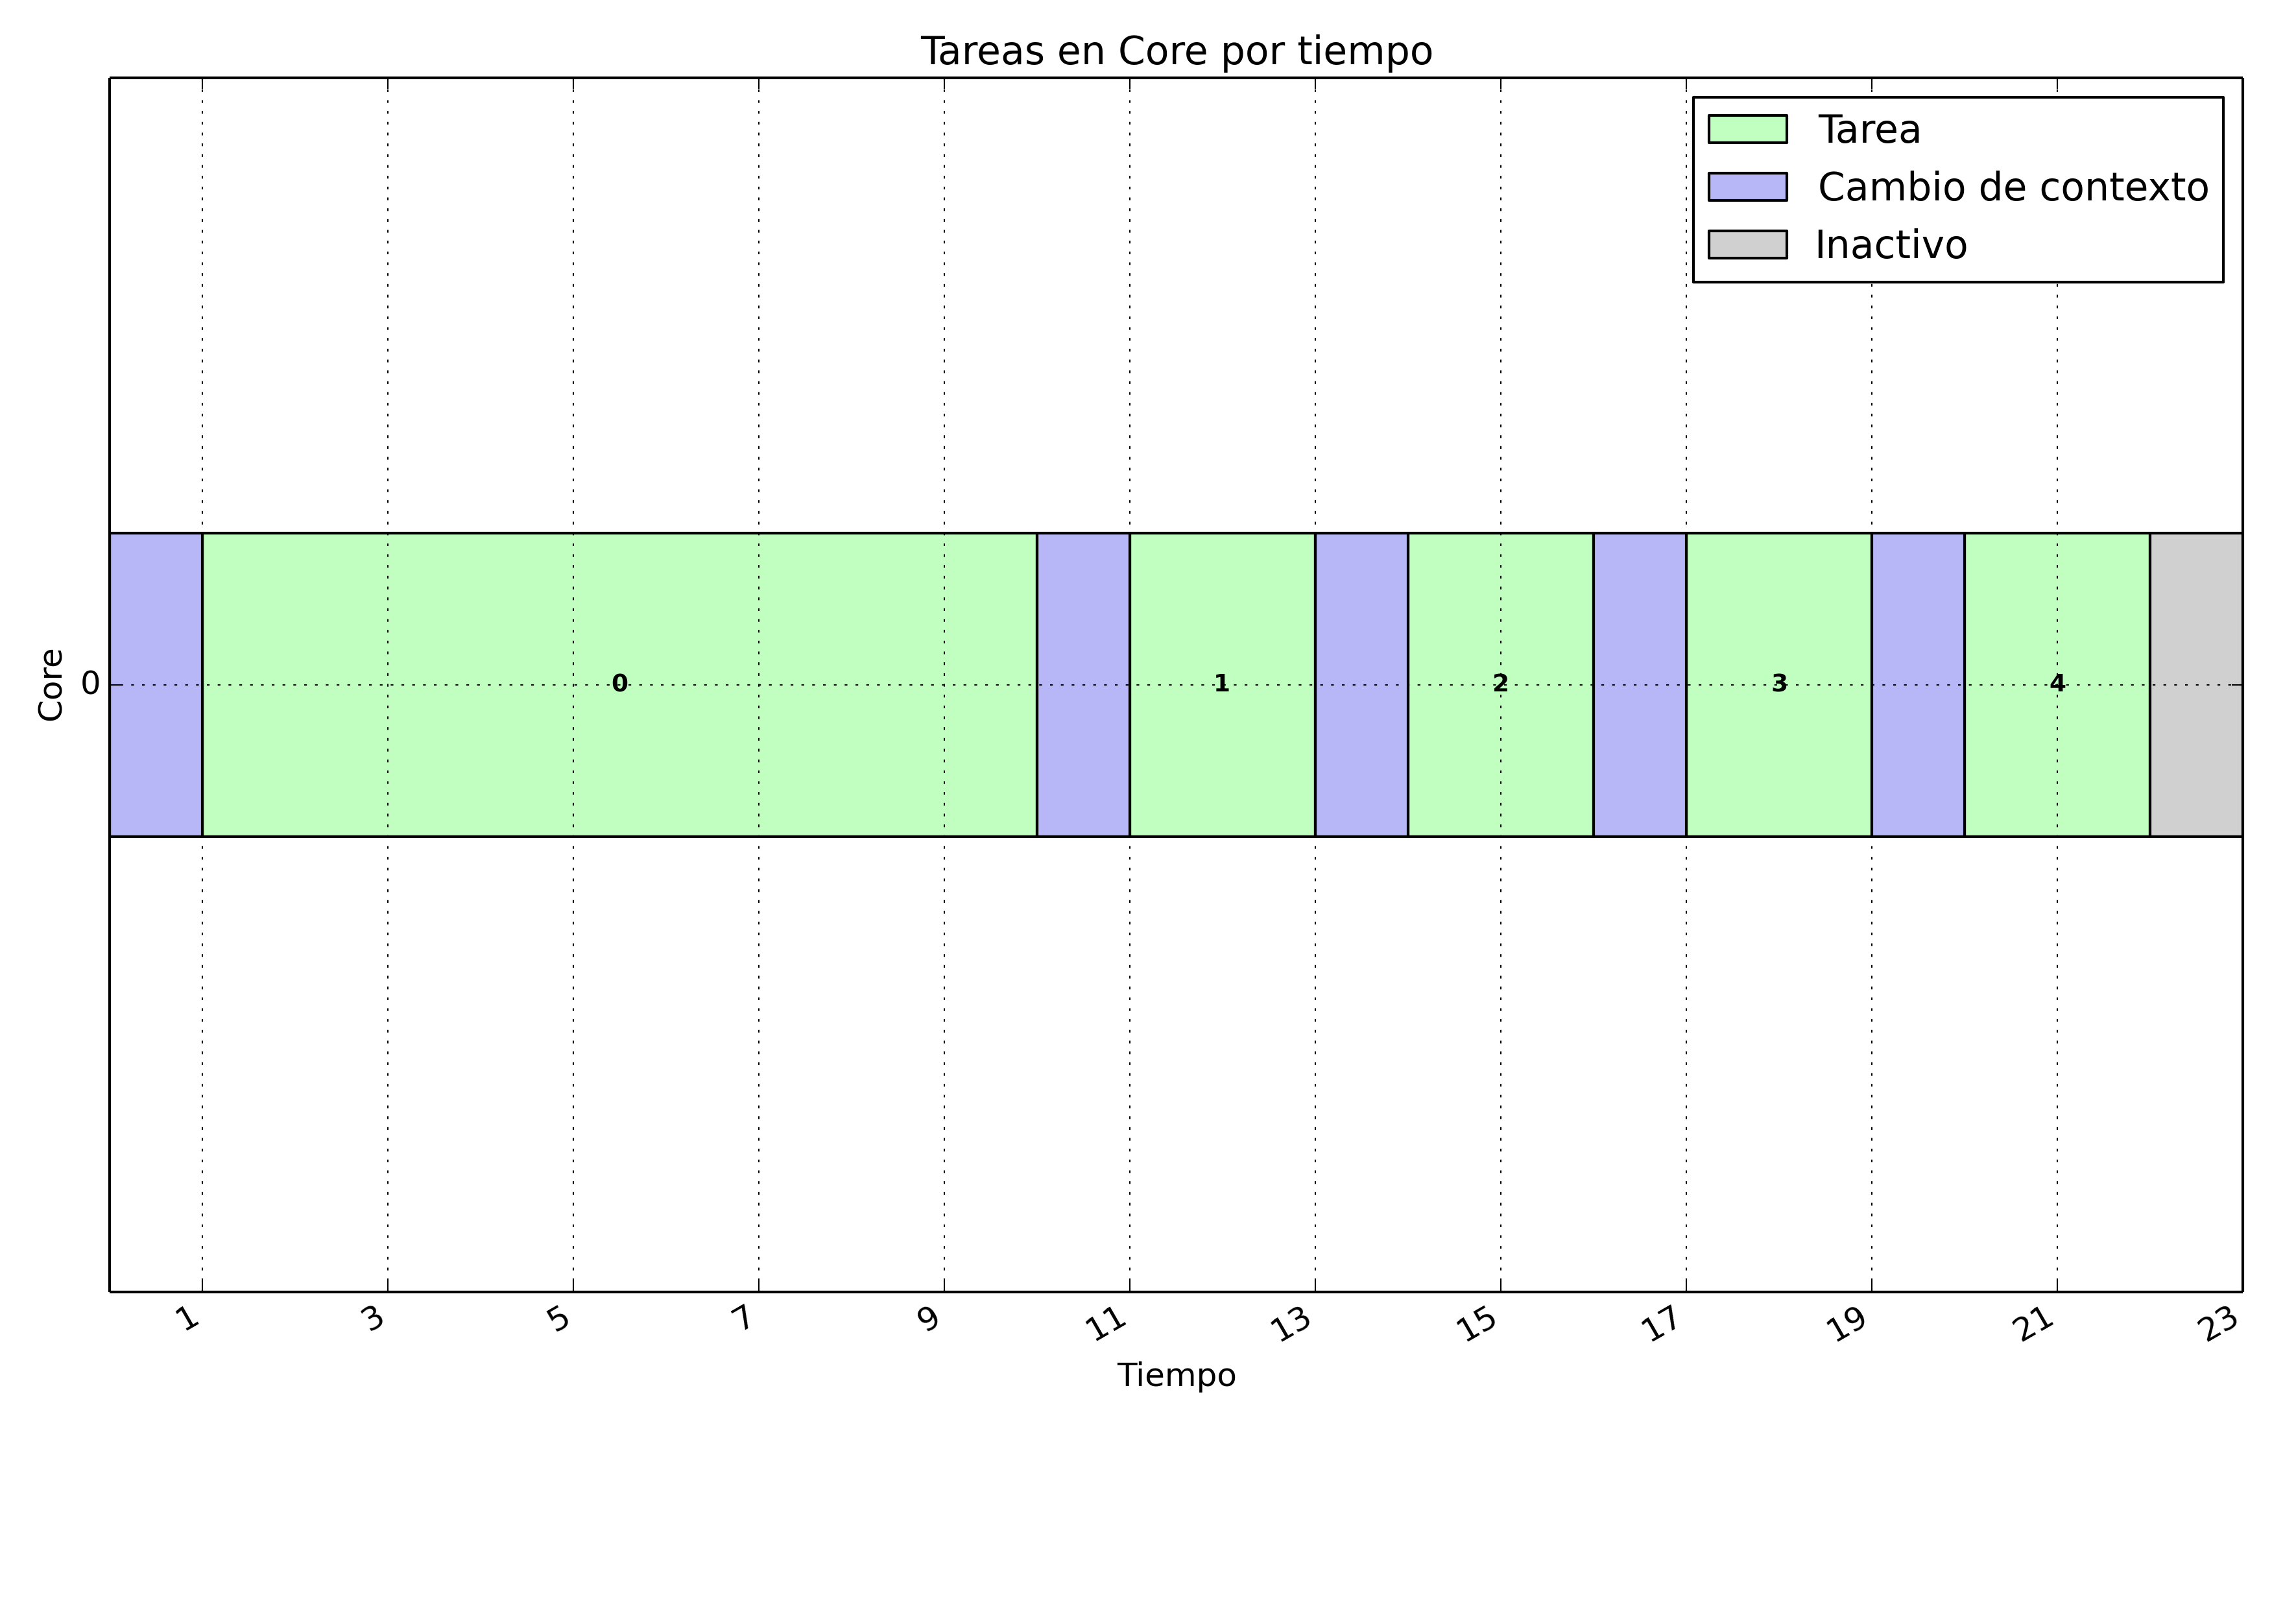
\includegraphics[width=\textwidth]{ejercicio_9_1}
\end{figure}

\begin{figure}[H]
\caption{Dynamic}
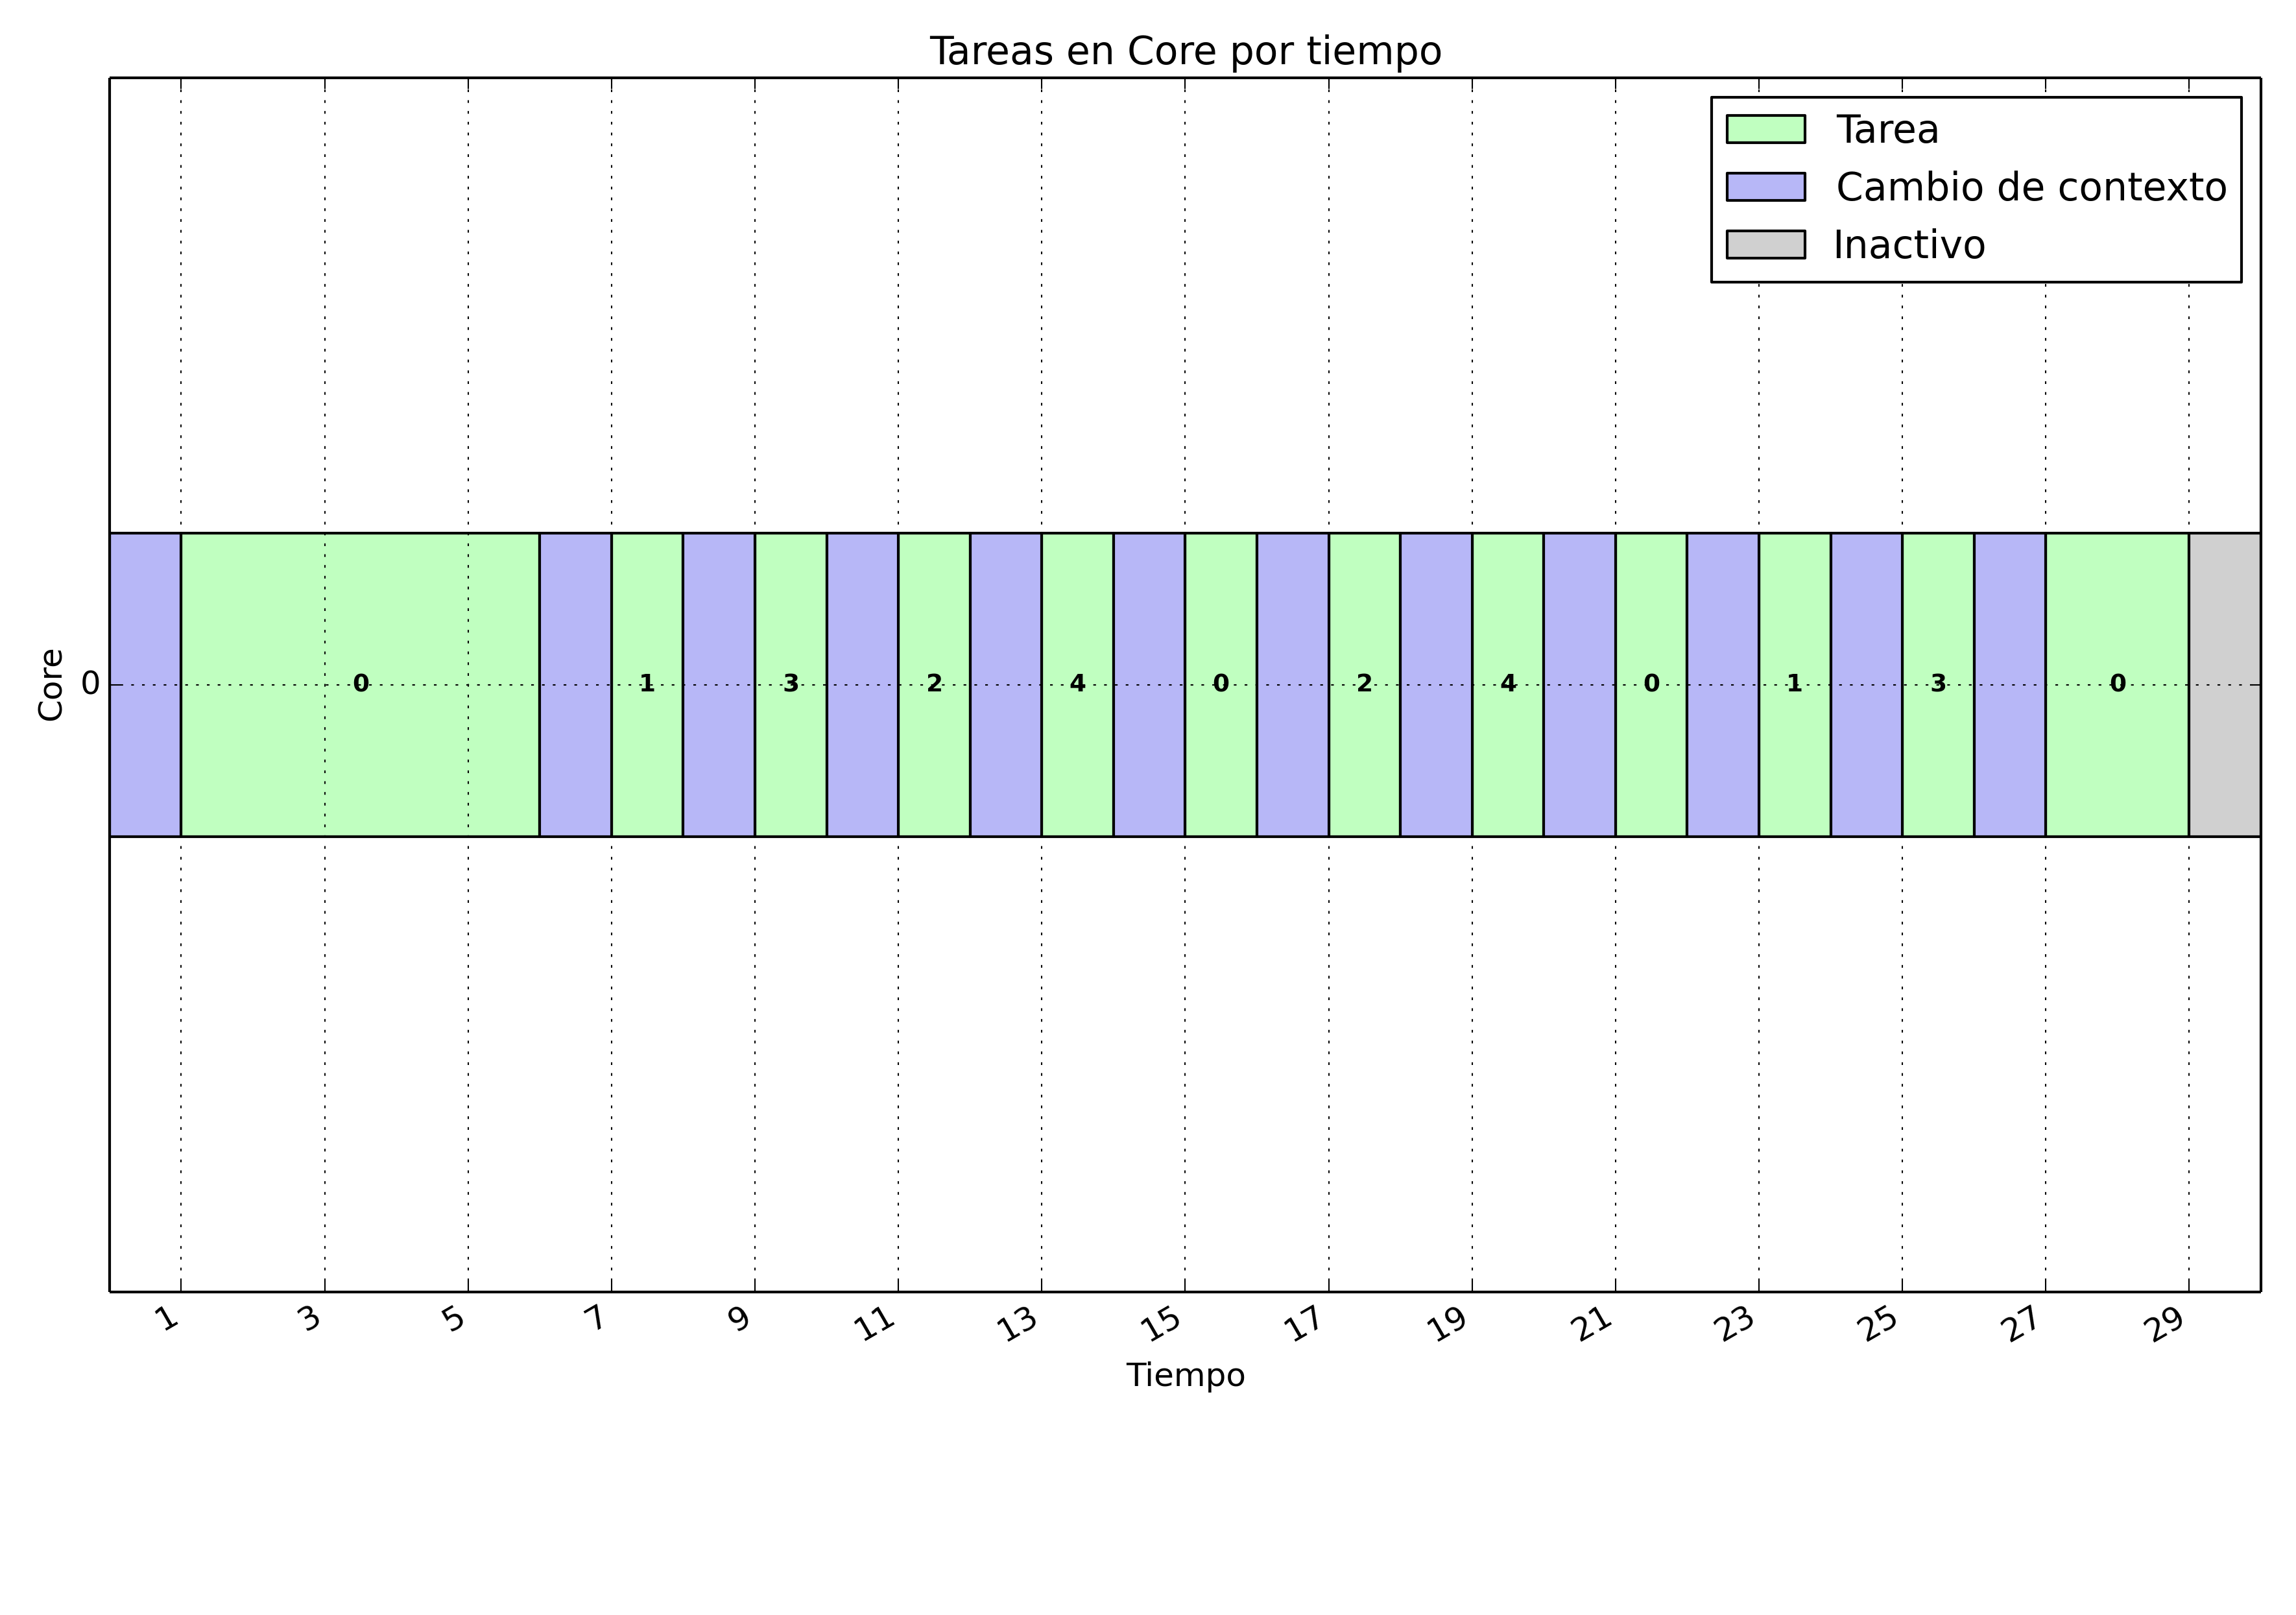
\includegraphics[width=\textwidth]{ejercicio_9_2}
\end{figure}

Se observa que en el caso del fixed se lleg\'o a un overflow para la tarea 0. Esto se produjo porque al ingresar las tareas de las familia B en el momento 6, fueron m\'as prioritarias en la medida en que ellas ten\'ian un request rate de $1/8$, mientras que el request rate de la tarea de la familia A era de $1/10$. 

Sin embargo, en el caso de la estrategia din\'amica no se produce el overflow porque al ingresar al sistema las tareas de la familia B, la tarea 0 sigue siendo m\'as prioritaria ya que su deadline se encuentra m\'as cercano.

\newpage
\section{Segunda Versi\'on de Round Robin}

La segunda versi\'on de round robin impide el pasaje de una tarea de un core a otro, de acuerdo a lo que requiere el \textbf{ejercicio 8}. De manera que en la carga del proceso se determina a qu\'e core tiene que estar asignado. El criterio para tomar esta decisi\'on se basa en la cantidad de tareas asociadas a un core: la nueva tarea que entra al sistema ir\'a a aquel core que tenga asignadas menos tareas en estado RUNNING o BLOCKED o READY.
Esta segunda versi\'on de \textit{round robin} se encuentra implementada en los archivos \verb+sched_rr2.h+ y \verb+sched_rr2.cpp+.

Para implementarla se us\'o un vector de colas. En el header \verb+sched_rr2.h+ se define este vector como un atributo privado.

Por otra parte, tenemos otro atributo privado, que guarda las tareas asignadas a cada core:

\begin{verbatim}
        std::vector< std::queue<int> > qs; // guarda las colas de prioridades asignadas 
                                           //a cada nucleo
        std::vector< std::vector<int> > nucleos; // guarda las tareas 
                                                 // asignadas a cada nucleo
\end{verbatim}

En el constructor del SchedRR2, inicializamos los vectores. Creamos tantas colas y vectores como cores existan en el ambiente:

\begin{verbatim}
SchedRR2::SchedRR2(vector<int> argn) {
	// Round robin recibe la cantidad de cores y sus cpu_quantum por parámetro
    unsigned int cantidadCores = argn[0];
    for (unsigned int i = 0; i < cantidadCores; i++) {
        queue<int> pids;
        vector<int> procesos;
        qs.push_back(pids);
        nucleos.push_back(procesos);
    }
}

\end{verbatim}

Cuando una tarea entra al sistema, se carga y se la asignamos al core que tiene menos tareas a\'no terminadas asociadas. Para ello iteramos por cada de las colas para ver cu\'al tiene menor cantidad:

\begin{verbatim}
    unsigned int nucleoMenosCongestionado = 0;
    unsigned int cantidadEnNucleoMenosCongestionado = qs[0].size();
    for (unsigned int i = 0; i < qs.size(); i++) { // se iteran todos los nucleos para ver
                        // cual es el menos congestionado
        if (qs[i].size() < cantidadEnNucleoMenosCongestionado) {
            nucleoMenosCongestionado = i;
            cantidadEnNucleoMenosCongestionado = qs[i].size();
        }
      }

     qs[nucleoMenosCongestionado].push(pid); // se pushea a este nucleo
      nucleos[nucleoMenosCongestionado].push_back(pid); // se lo asocia al nucleo                         
      //menos congestionado

\end{verbatim}

La selecci\'on para la siguiente tarea a ejecutarse, es similar a SchedRR, con la diferencia de que se consideran solamente la cola asociada al core que envi\'o la interrupci\'on de reloj. Lo mismo ocurre en el caso del desbloqueo. La tarea se vuelve a asociar a la cola a la que se vincul\'o en el momento de la carga.

La otra diferencia a tener en cuenta es que cuando una tarea termina, no solamente se desencola sino que se elimina del vector que tiene las tareas asociadas al core en donde culmin\'o su ciclo de vida.

El primer experimento que hicimos consiste en ejecutar el siguiente lote de tareas:

\begin{verbatim}
TaskCPU 3
TaskCPU 3
TaskCPU 3
TaskCPU 3
TaskCPU 3
\end{verbatim}

con 2 cores, tomando como overhead de cambio de core 1, 2, 3 y 4 quantums. El tiempo de cambio de contexto se mantuvo en 1 en cada una de las mediciones. Se hizo este experimento para verificar c\'omo incid\'ia el cambio del overhead de cambio de core. 


\begin{figure}[H]
\caption{SchedRR 5 TaskCPU 2 cores 1, 2, 3, 4 para cambio de core}
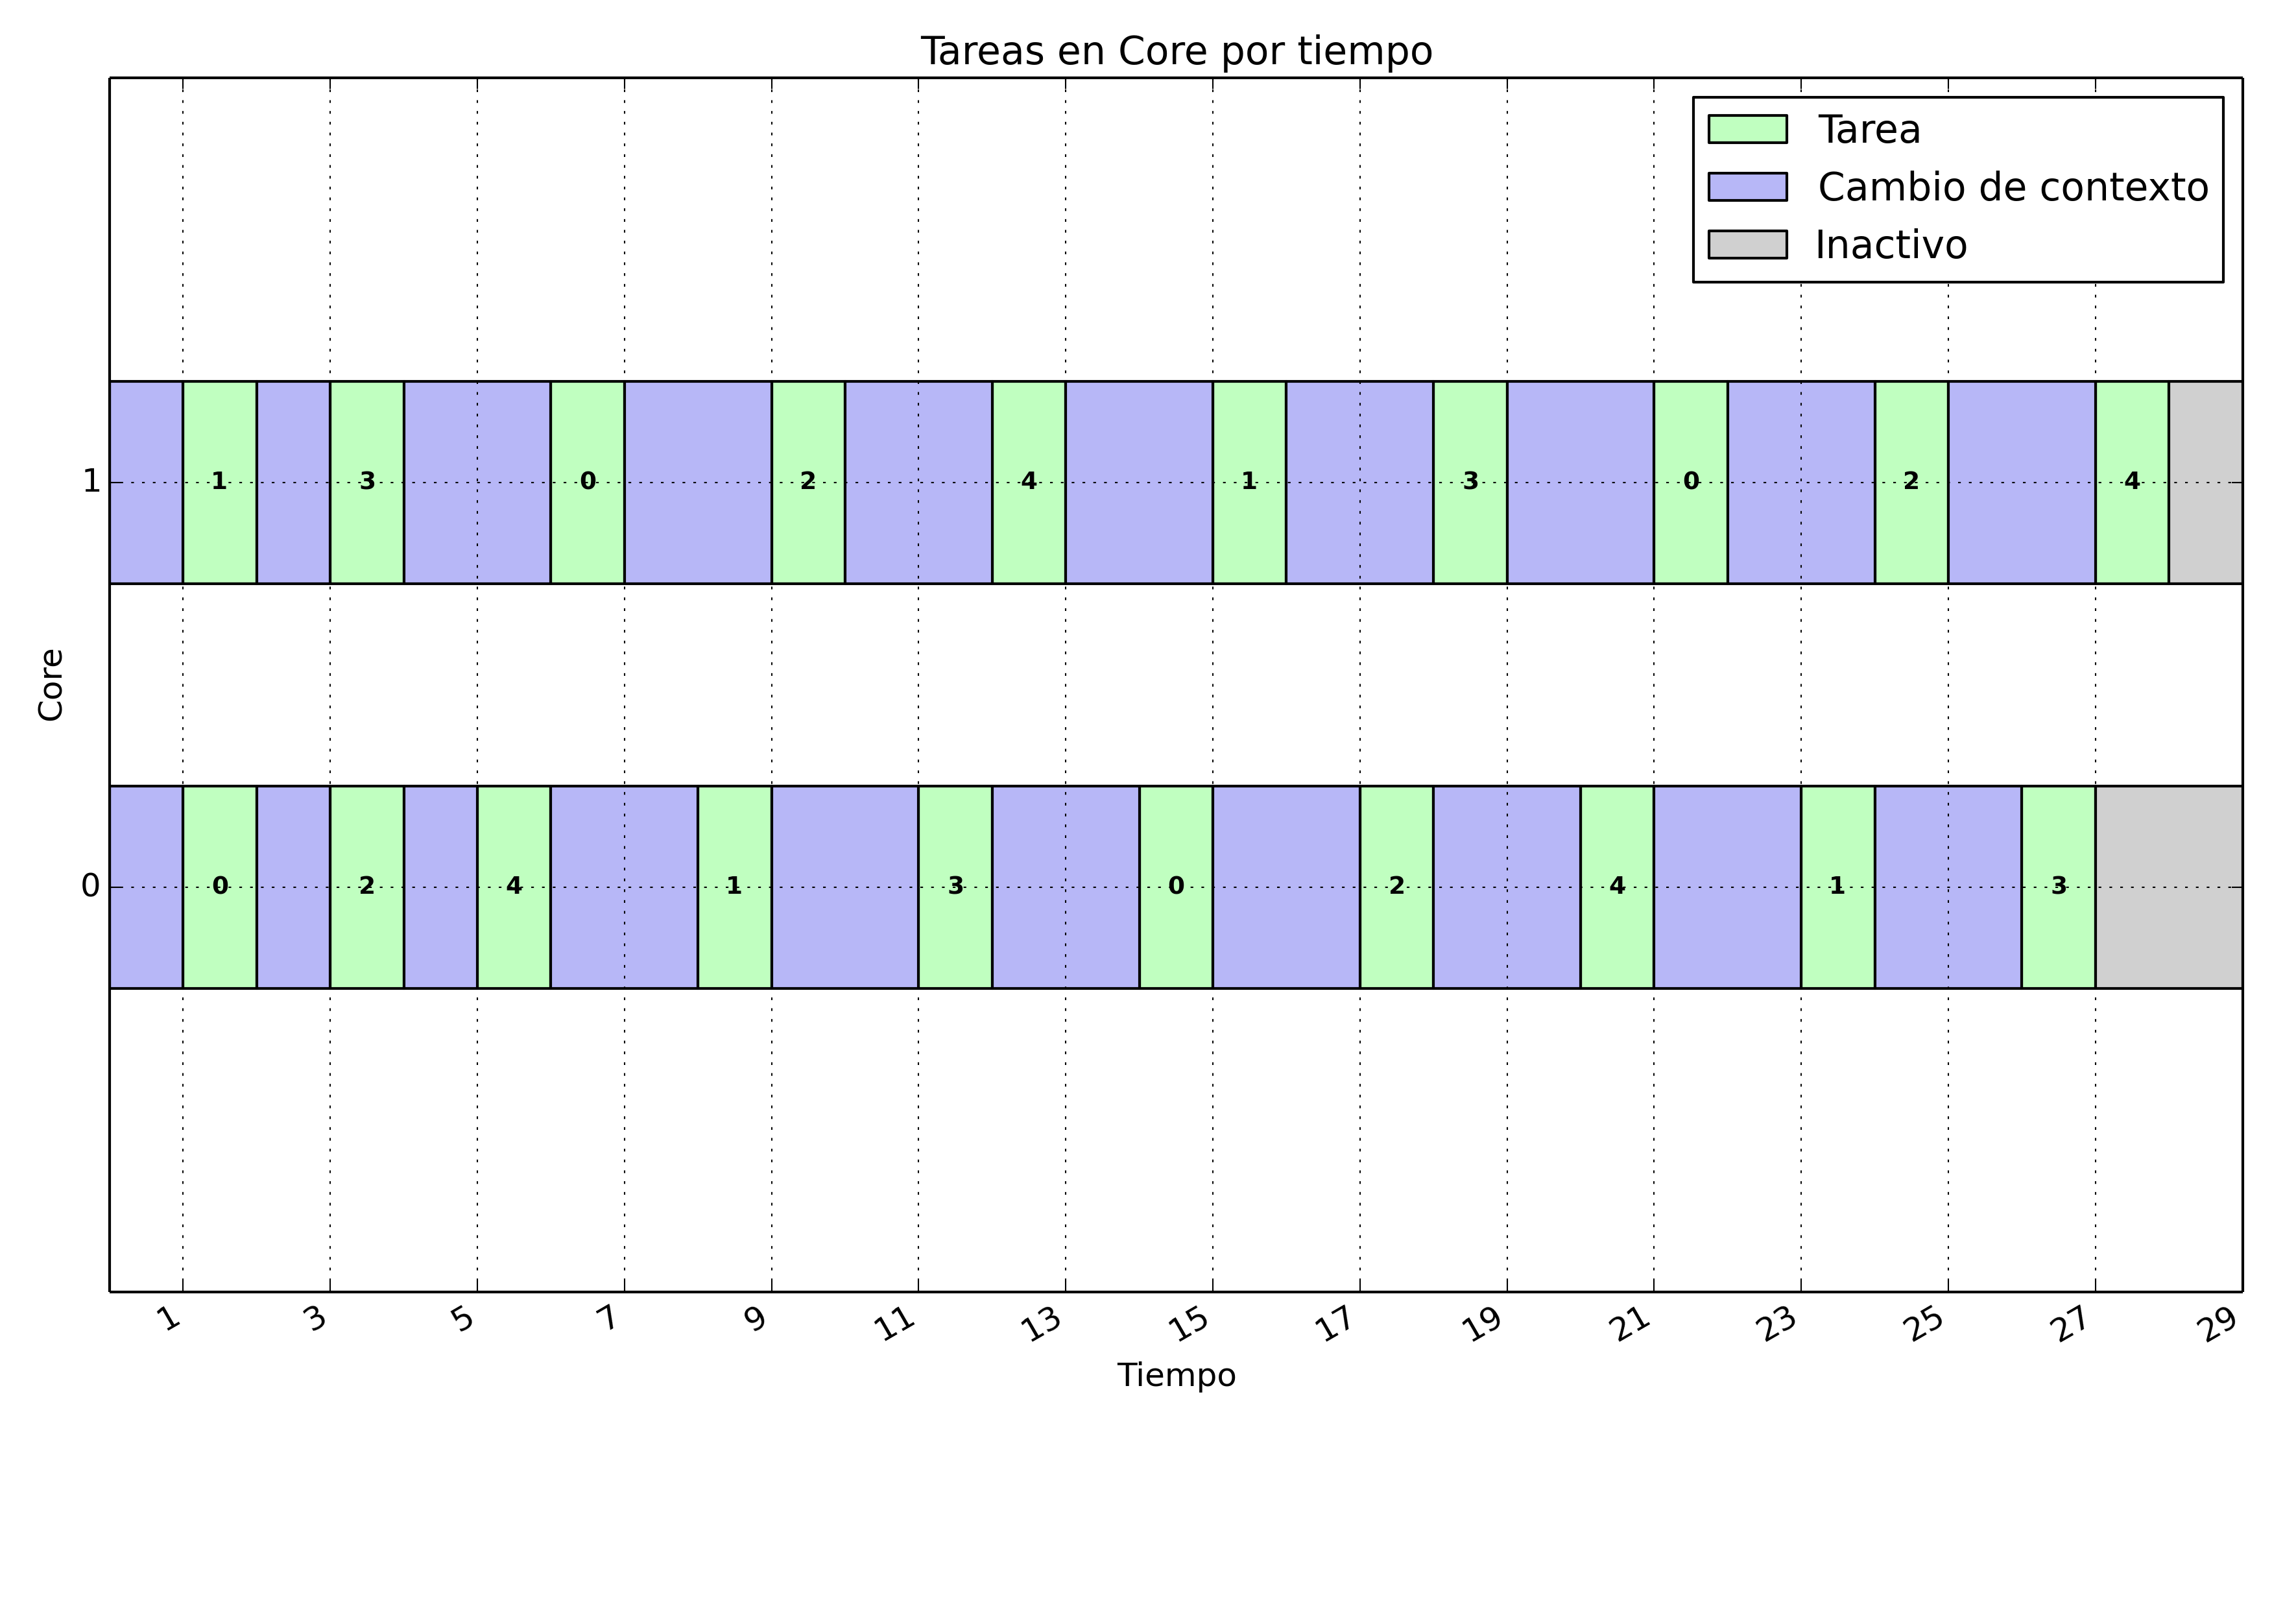
\includegraphics[width=\textwidth]{ejercicio_8_1}
\end{figure}

\begin{figure}[H]
\caption{SchedRR2 5 TaskCPU 2 cores 1 para cambio de core}
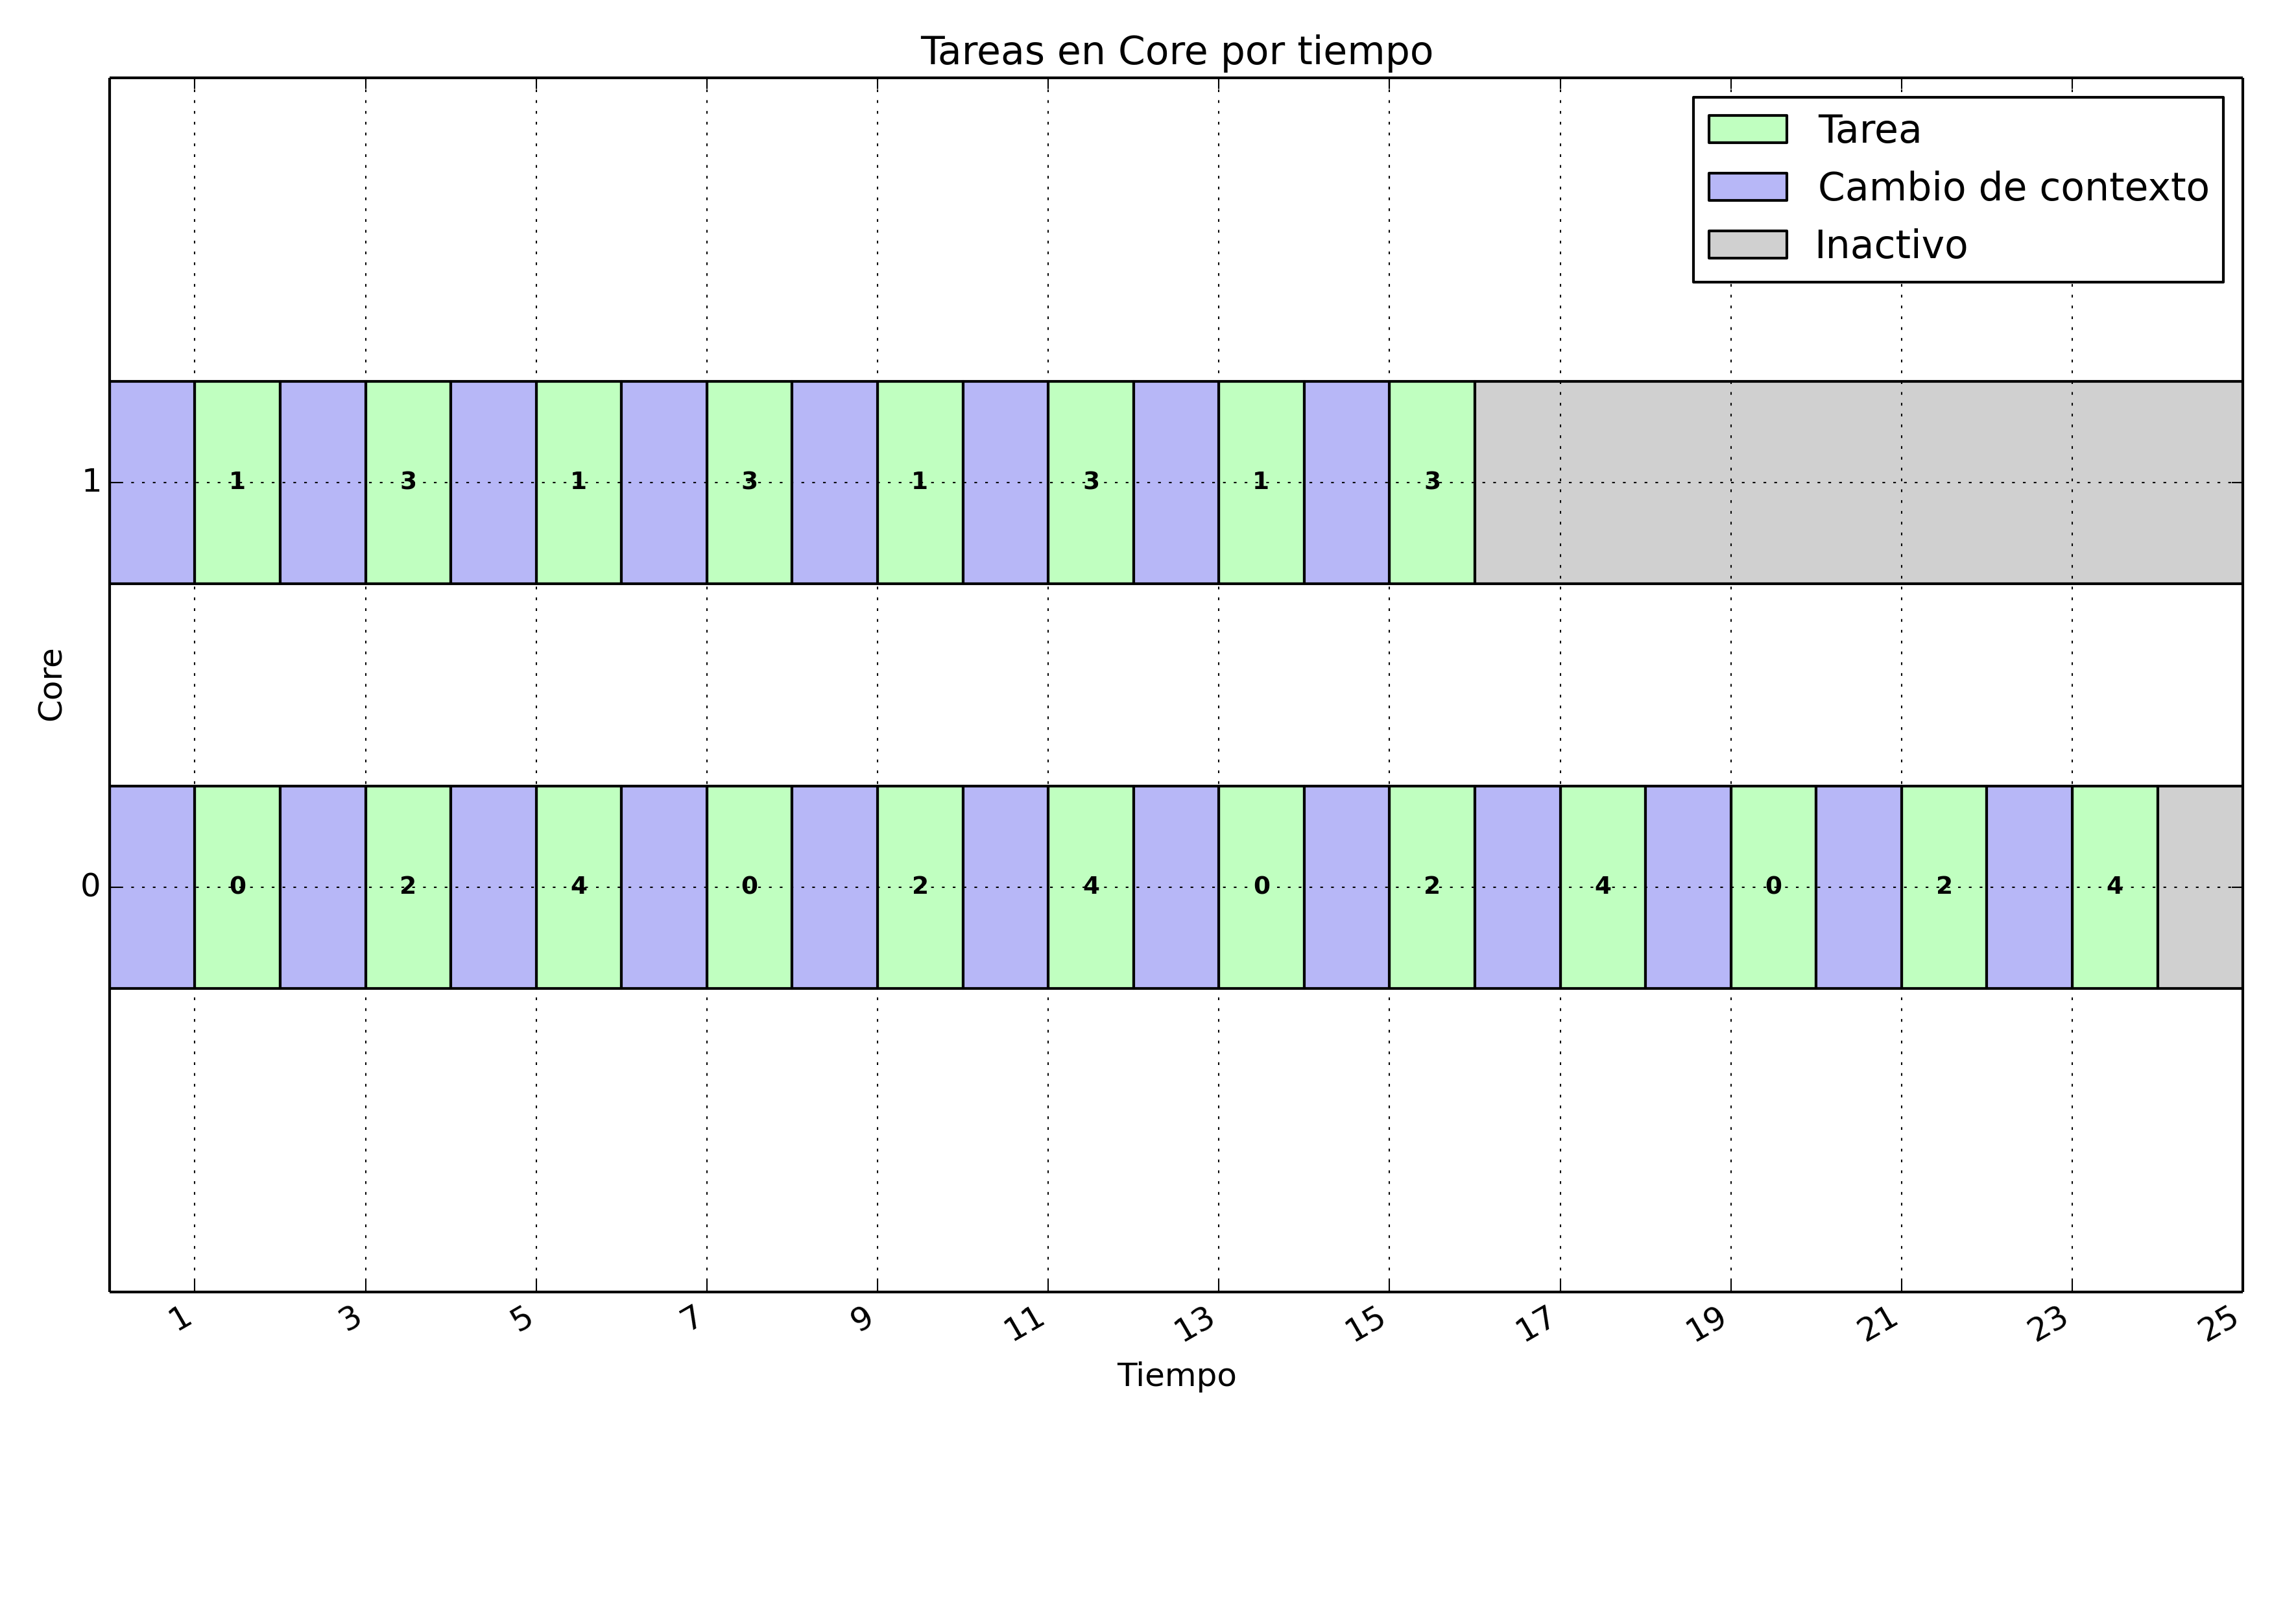
\includegraphics[width=\textwidth]{ejercicio_8_2}
\end{figure}


\begin{figure}[H]
\caption{SchedRR2 5 TaskCPU 2 cores 2 para cambio de core}
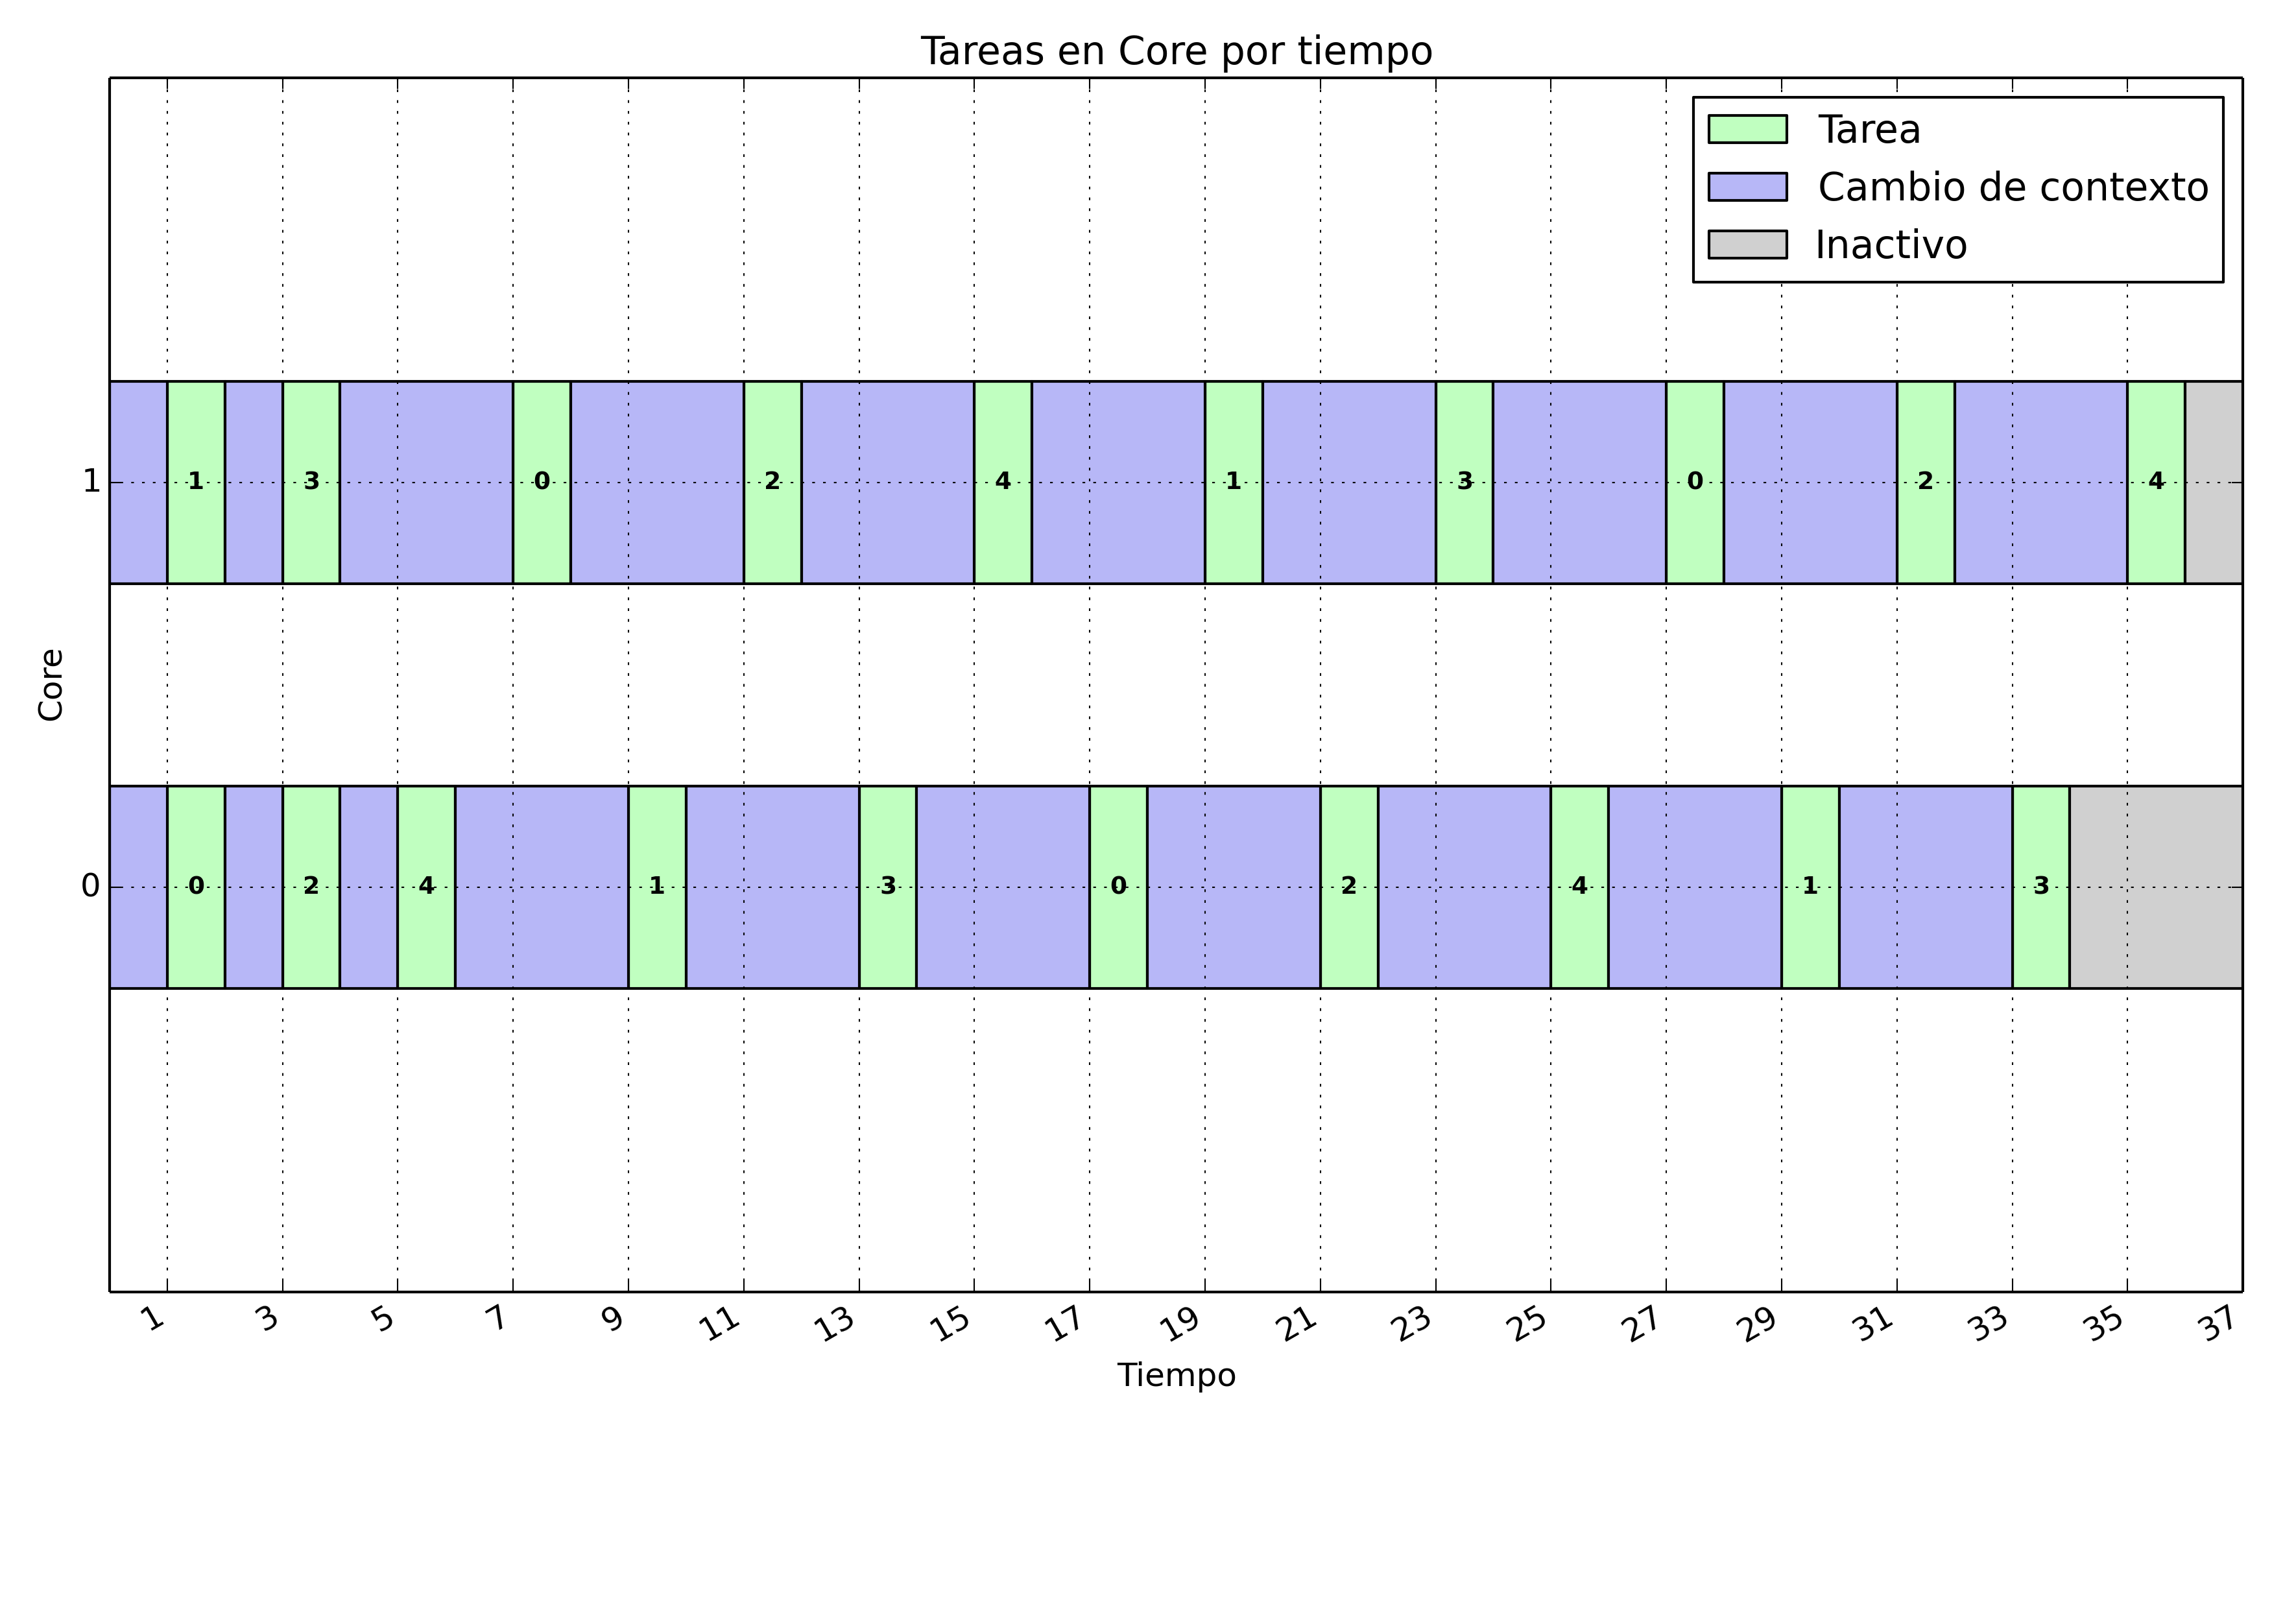
\includegraphics[width=\textwidth]{ejercicio_8_3}
\end{figure}


\begin{figure}[H]
\caption{SchedRR2 5 TaskCPU 2 cores 3  para cambio de core}
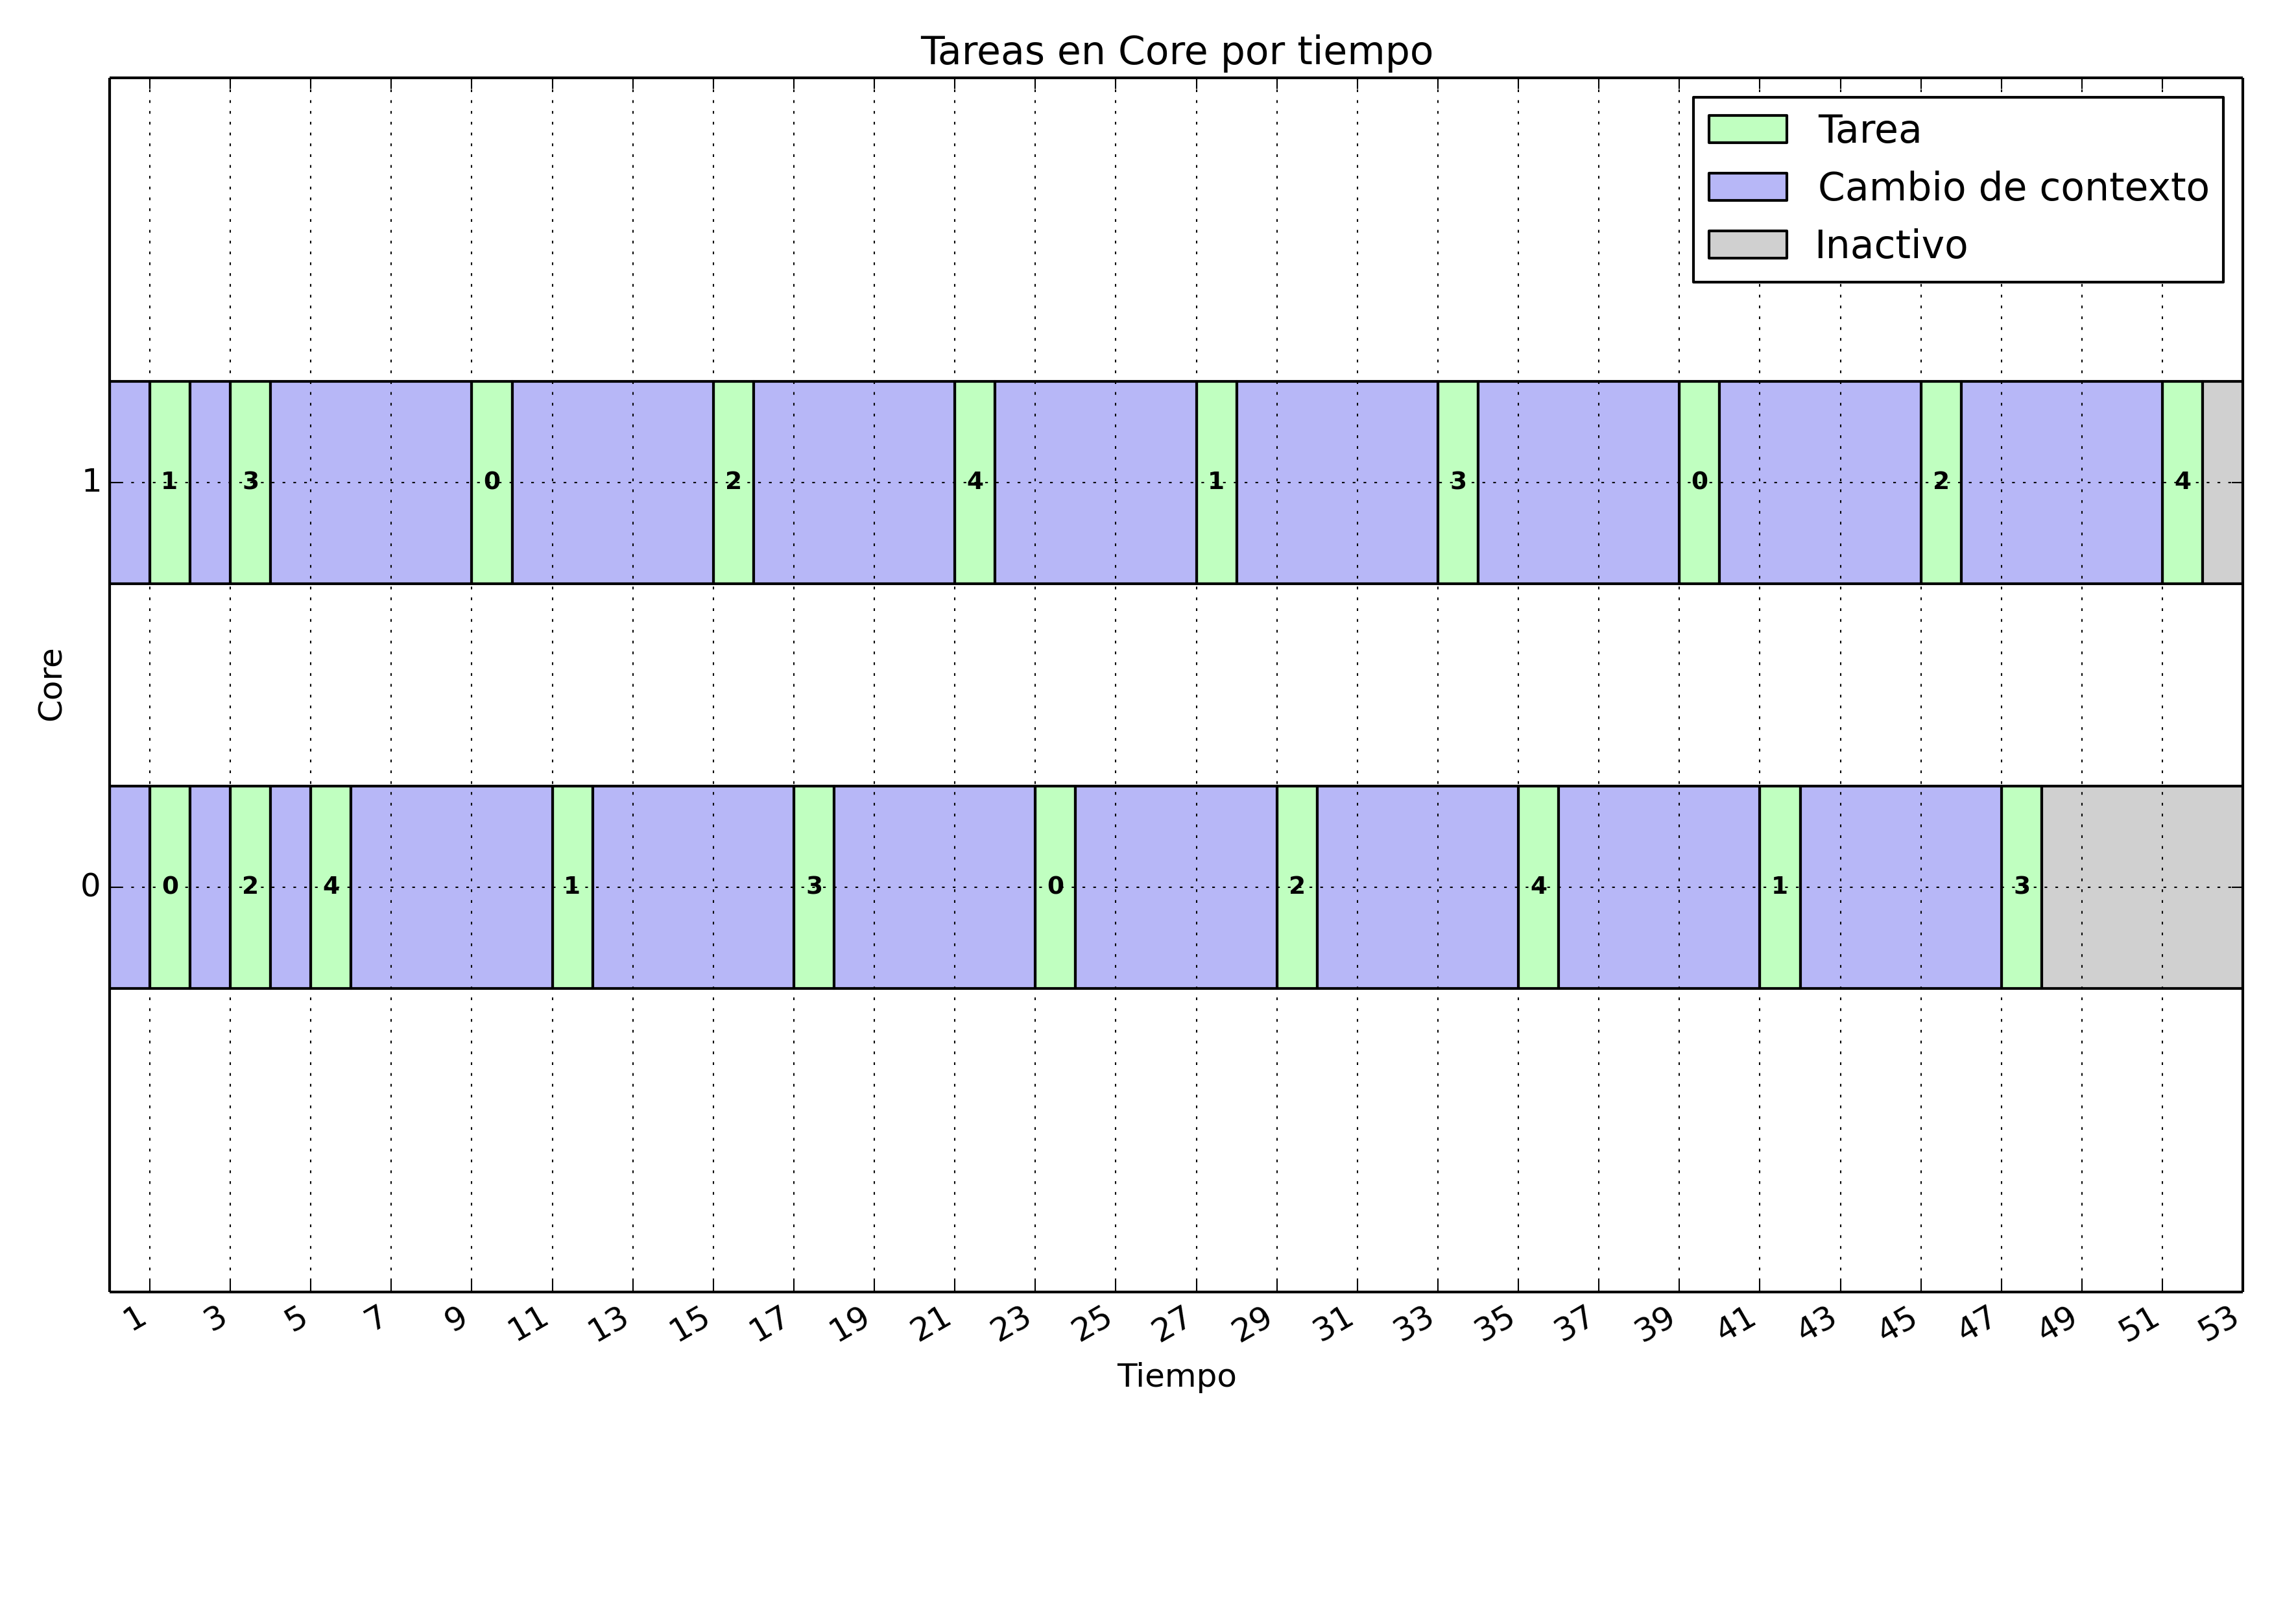
\includegraphics[width=\textwidth]{ejercicio_8_4}
\end{figure}

Se observa que el tiempo de turnaround promedio va aumentando en la medida en que aumenta el costo del cambio de core para SchedRR, mientras que en SchedRR2 se mantiene estable, ya que cada una de las tareas se mantiene asociada a una cola.
 

\newpage

\begin{thebibliography}{9}

\bibitem{stallings2008}
  William Stallings,
  \emph{Operating Systems},
  Prentice Hall, Upper Saddle River
  2008.

\bibitem{tanenbaum2001}
  Andrew S. Tanenbaum,
  \emph{Modern operating systems},
  Prentice Hall, Upper Saddle River
  2001.

\bibitem{liuleiland1973}
  C. L. Liu y James W. Layland,
  \emph{Scheduling Algorithms for Multiprogramming in a Hard-Real-Time Environment},  Journal of the ACM  (JACM), 1973.

\end{thebibliography}

\end{document}
